%% Exemplo de utilizacao do estilo de formatacao normas-utf-tex (http://normas-utf-tex.sourceforge.net)
%% Autores: (200?-2011) Hugo Vieira Neto (hvieir@utfpr.edu.br)
%%          (200?-2011) Diogo Rosa Kuiaski (diogo.kuiaski@gmail.com)
%%          (2011-2012) Marcos Talau <talau@users.sourceforge.net>
%% Colaborador:
%%          (2011) César M. Vargas Benitez <cesarvargasb@gmail.com>

\documentclass[openright]{normas-utf-tex} %openright = o capitulo comeca sempre em paginas impares
%\documentclass[oneside]{normas-utf-tex} %oneside = para dissertacoes com numero de paginas menor que 100 (apenas frente da folha) 

% force A4 paper format
\special{papersize=210mm,297mm}

\usepackage[alf,abnt-emphasize=bf,bibjustif,recuo=0cm, abnt-etal-cite=2, abnt-etal-list=99]{abntcite} %configuracao correta das referencias bibliograficas.

\usepackage[brazil]{babel} % pacote portugues brasileiro
\usepackage[utf8]{inputenc} % pacote para acentuacao direta
\usepackage{amsmath,amsfonts,amssymb} % pacote matematico
\usepackage{graphicx} % pacote grafico
\usepackage{times} % fonte times
\usepackage[final]{pdfpages} % adicao da ata
\usepackage{epigraph}
\usepackage{chngcntr}
%\usepackage{subfigure}
\usepackage{caption}
\usepackage{subcaption}

%Podem utilizar GEOMETRY{...} para realizar pequenos ajustes das margens. Onde, left=esquerda, right=direita, top=superior, bottom=inferior. P.ex.:
%\geometry{left=3.0cm,right=1.5cm,top=4cm,bottom=1cm} 

% ---------- Preambulo ----------
\instituicao{Universidade Tecnológica Federal do Paraná}
\programa{Programa de Pós-Graduação em Engenharia Elétrica e Informática Industrial}
%\area{}

\documento{Dissertação}
\nivel{Mestrado}
\titulacao{Mestre}

\titulo{{Título em português}} % titulo do trabalho em portugues
\title{\MakeUppercase{Title in English}} % titulo do trabalho em ingles

\autor{Daniel Alexandre Oleinik} % autor do trabalho
\cita{OLEINIK, Daniel Alexandre} % sobrenome (maiusculas), nome do autor do trabalho

\palavraschave{\emph{Smart Grid}, Chaveador óptico, Redes IP, Redes \emph{Mesh}, Otimização, Latência, Algoritmos Genéticos} % palavras-chave do trabalho
\keywords{\emph{Smart Grid, Optical Switch, IP networks, Mesh networks, Optimization, Latency, Genetic Algorithms}} % palavras-chave do trabalho em ingles

\comentario{Dissertação apresentada ao Programa de Pós-graduação em Engenharia Elétrica e Informática Industrial da Universidade Tecnológica Federal do Paraná como requisito parcial para obtenção do grau ``Mestre em Ciências'' - Área de Concentração: Informática Industrial}

\orientador{Mauro Sergio Pereira Fonseca} % nome do orientador do trabalho
%\orientador[Orientadora:]{Nome da Orientadora} % <- no caso de orientadora, usar esta sintaxe
%\coorientador{Nome do Co-orientador} % nome do co-orientador do trabalho, caso exista
%\coorientador[Co-orientadora:]{Nome da Co-orientadora} % <- no caso de co-orientadora, usar esta sintaxe
%\coorientador[Co-orientadores:]{Nome do Co-orientador} % no caso de 2 co-orientadores, usar esta sintaxe
%\coorientadorb{Nome do Co-orientador 2}	% este comando inclui o nome do 2o co-orientador

\local{Curitiba} % cidade
\data{\the\year} % ano automatico

% desativa hifenizacao mantendo o texto justificado.
% thanks to Emilio C. G. Wille
\tolerance=1
\emergencystretch=\maxdimen
\hyphenpenalty=10000
\hbadness=10000
\sloppy

%---------- Inicio do Documento ----------
\begin{document}

\capa % geracao automatica da capa
\folhaderosto % geracao automatica da folha de rosto

% Lembre-se de que a ficha catalografica eh impressa no verso da folha de rosto
% Ficha catalografica
\fichacatpum{T137}
\fichacatautor{Sobrenome, Nome}
\fichacatpgbib{\pageref{bibstart}-\pageref{bibend}}
\fichacatpalcha{1. Teoria do controle. 2. Redes de comutação. 3. TCP/IP (Protocolo de rede de computação), ...}
\fichacatpdois{CDD (22. ed.) 621.3}
\fichacatbib{Biblioteca Dois Vizinhos}
\fichacat

% insercao da ATA
%\includepdf{ata.pdf}

% dedicatoria
%\begin{dedicatoria}
%Texto da dedicatória.
%\end{dedicatoria}
%
%% agradecimentos (opcional)
%\begin{agradecimentos}
%Texto dos agradecimentos.
%\end{agradecimentos}

% epigrafe (opcional)
\begin{epigrafe}
\epigraph{\emph{``Muito melhor é o homem paciente que o guerreiro, mais vale controlar as emoções e os ímpetos do que conquistar toda uma cidade!''}}{Provérbios 16:32}
\end{epigrafe}

%resumo
\begin{resumo}
O crescente consumo de energia proveniente de fontes não renováveis e finitas vem incentivando o avanço no desenvolvimento e utilização de novas opções de geração de energia. Estas opções, quando incorporadas ao sistema atual de geração e distribuição de energia elétrica, devem demandar novas exigências do sistema de comunicação utilizado entre os equipamentos da rede, motivando o desenvolvimento do \emph{Smart Grid} (SG). O presente documento propõe um método para melhoria e otimização de uma rede, ou grid, de acesso construída em fibra óptica com topologia \emph{mesh}, através de alterações das conexões físicas da rede em conjunto com uma gerência reativa inteligente.
\end{resumo}

%abstract
\begin{abstract}
The increasing consumption of energy from nonrenewable and finite sources is encouraging the advance of development and use
of new energy generation options. These options, when incorporated into the current electricity generation and distribution system,
should demand new requirements from the communication system used to provide the communication link between the network
equipment used, motivating the development of Smart grid. This document proposes a method to improve and optimize the network
or grid access, built with optic fiber and mesh topology through the handling of the physical connections in the network together with
a smart reactive management.
\end{abstract}

% listas (opcionais, mas recomenda-se a partir de 5 elementos)
\listadefiguras % geracao automatica da lista de figuras
\listadetabelas % geracao automatica da lista de tabelas
\listadequadros % adivinhe :)
\listadesiglas % geracao automatica da lista de siglas
\listadesimbolos % geracao automatica da lista de simbolos

% sumario
\sumario % geracao automatica do sumario


%---------- Inicio do Texto ----------
% recomenda-se a escrita de cada capitulo em um arquivo texto separado (exemplo: intro.tex, fund.tex, exper.tex, concl.tex, etc.) e a posterior inclusao dos mesmos no mestre do documento utilizando o comando \input{}, da seguinte forma:
%\input{intro.tex}
%\input{fund.tex}
%\input{exper.tex}
%\input{concl.tex}


\setcounter{page}{12}

%---------- Primeiro Capitulo ----------
\input{introducao.tex}

\counterwithout{figure}{chapter}% Continuous numbering of figures
%---------- Segundo Capitulo ----------
\chapter{Fundamentação Teórica}
Este capítulo apresenta conceitos utilizados no desenvolvimento do trabalho, e portanto necessários para o correto entendimento do mesmo.

\section{Redes de Computadores}
A história dos computadores de grande escala começa em fevereiro de 1946 através da invenção do primeiro ``computador integrador numérico eletrônico'' \sigla{ENIAC}{\emph{Electronic Numerical Integrator and Computer}} \cite{Book-Jean2013}. Ele começou a ser desenvolvido anos antes, durante a Segunda Guerra Mundial, com a principal tarefa de auxiliar nos cálculos necessários para o fronte de batalha.

Em meados dos anos 50, com a popularização dos transistores, foi possível realizar uma imensa miniaturização dos circuitos eletrônicos possibilitando a criação de máquinas com altíssimo poder de processamento em um tamanho extremamente reduzido. Além disso, essas máquinas tornaram-se cada vez mais robustas e baratas, fazendo com que a posse e utilização de computadores pudesse ser disseminada alcançando os patamares atuais.

Neste sentido foi natural a necessidade da troca de informações/dados entre os diversos computadores existentes, o que claramente não representa maiores problemas caso os equipamentos em questão estejam fisicamente perto uns dos outros. Em contrapartida, é fácil imaginar a dificuldade de realização desta tarefa no caso em que estes equipamentos estão fisicamente distantes. Este é o cerne do problema que motivou a criação das redes de computadores.

Segundo \cite{Book-Kurose2013} uma rede de computadores nada mais é do que uma infraestrutura de comunicação que fornece serviços à aplicações distribuídas através de \emph{links} de comunicação contendo ``chaveadores de pacotes''. Sendo que uma rede pode ser essencialmente definida por seu tamanho, topologia e tecnologia de transmissão utilizada \cite{Book-Tanenbaum2003}. 
%Essas características, apesar de presentes em qualquer rede, são especialmente aplicáveis a redes locais (comumente chamadas de \sigla{LAN}{\emph{Local Area Network}}). 

\subsection{Tamanho}
Segundo \cite{Book-Tanenbaum2003} uma \sigla{LAN}{\emph{Local Area Network}} ou Rede Local possui tamanho restrito, e por isso seu desempenho é previsível. Ou seja, os piores tempos de transmissão de pacotes são conhecidos. 

Este tipo de rede pode possuir diversas topologias diferentes e pode ser encontrada nas mais diversas aplicações, desde residenciais, até industriais ou de automação. Uma das suas principais vantagens é a previsibilidade em termos de latência, visto que além de limitada e completamente conhecida ela normalmente não sofre alterações frequentes.

Uma Rede Metropolitana ou \sigla{MAN}{Metropolitan Area Network}, por sua vez, abrange uma cidade. Redes como esta foram inicialmente instaladas para sinais de TV a cabo. Atualmente elas são também utilizadas por provedores de internet \cite{Book-Tanenbaum2003}.

Uma Rede Geograficamente Distribuída ou \sigla{WAN}{Wide Area Network} abrange uma grande região como um país ou um continente e é responsável pelo roteamento dos pacotes entre as redes origem e destino. A forma e caminho utilizados para enviar as informações neste processo depende do algoritmo de roteamento utilizado. \cite{Book-Tanenbaum2003}

\subsection{Topologia}
Existem diversas formas de realizar a interconexão entre \emph{hosts} (dispositivos finais ou \emph{endpoints}). A topologia da rede depende de como esta interconexão é realizada. De maneira geral, podem-se destacar como mais comuns as topologias em barramento, anel, estrela, árvore e \emph{mesh}.

Uma topologia em barramento compartilha um mesmo meio para diversos \emph{hosts}. Todas as vezes que um deles deseja enviar alguma informação todos os equipamentos a recebem mas apenas o destinatário final à utiliza. Visto que o meio de comunicação é compartilhado é necessário existir alguma política de controle de acesso ao meio, prevenindo que mais de um \emph{endpoint} envie dados ao mesmo tempo, o que poderia gerar uma ``colisão'' embaralhando os dados de ambas as fontes. Este controle fica sob responsabilidade do protocolo de comunicação utilizado. A Figura \ref{fig_topologia_multiplo_barramento} representa uma rede conectada em barramento, percebe-se que o barramento central é compartilhado entre os diversos dispositivos conectados.

%\begin{figure}[!htb]
	%\centering
	%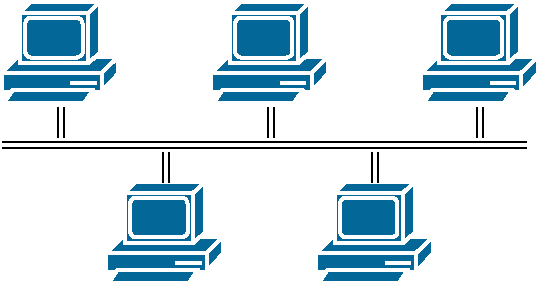
\includegraphics[width=0.2\textwidth]{./figuras/Topologia-Barramento.pdf} % <- formatos PNG, JPG e PDF
	%\caption[Exemplo de topologia em barramento]{Exemplo de topologia conectada em barramento. Percebe-se que o barramento central é compartilhado entre os diversos dispositivos conectados.}
	%\label{fig_topologia_barramento}
%\end{figure}

Na topologia em anel os \emph{hosts} são conectados através de um \emph{link} fechado, criando um anel. Cada estação é responsável por receber os dados em uma porta e encaminhá-los à outra até que este alcance seu destino. Neste tipo de topologia as colisões de dados são menos frequentes, visto que cada ``perna'' do \emph{link} é estabelecida entre apenas dois \emph{hosts}, em contrapartida o protocolo utilizado precisa tratar a dinâmica de recepção e retransmissão de dados entre todos os \emph{links}. Este tipo de rede fornece redundância já que as mensagens trocadas podem ser enviadas por mais de um caminho. A Figura \ref{fig_topologia_multiplo_barramento_anel} representa uma rede em anel, pode-se perceber que neste caso todos os equipamentos fazem parte da rede e precisam repetir os dados recebidos para os demais.

%\begin{figure}[!htb]
	%\centering
	%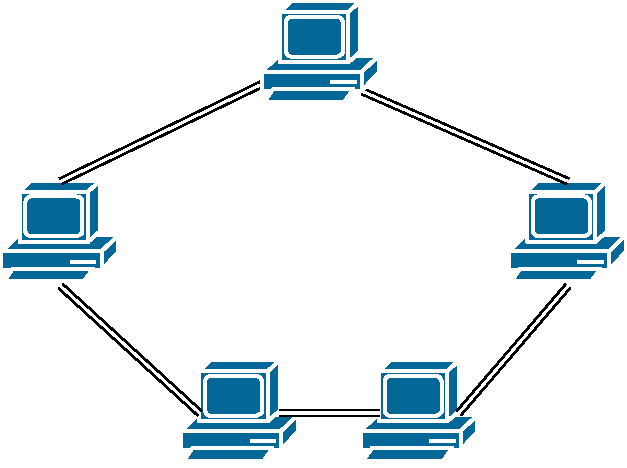
\includegraphics[width=0.2\textwidth]{./figuras/Topologia-Anel.pdf} % <- formatos PNG, JPG e PDF
	%\caption[Exemplo de topologia em anel]{Exemplo de topologia conectada em anel. Percebe-se que todos os equipamentos fazem parte da rede e precisam repetir os dados recebidos para os demais.}
	%\label{fig_topologia_anel}
%\end{figure}

A topologia estrela é muito utilizada em redes sem fio, visto que de maneira geral, todos os \emph{hosts} estão conectados a um ponto de acesso ou \sigla{AP}{Access Point}. Esse tipo de rede também pode ser facilmente encontrada em um meio cabeado, como no caso da utilização dos roteadores/switches residenciais, onde todos os \emph{hosts} são conectados a um mesmo equipamento responsável pela criação de uma LAN e interconexão com uma WAN. A Figura \ref{fig_topologia_multiplo_estrela} representa uma rede de topologia estrela, neste tipo de topologia todos os equipamentos estão ligados a um nó central, neste caso um \emph{switch}.

%\begin{figure}[!htb]
	%\centering
	%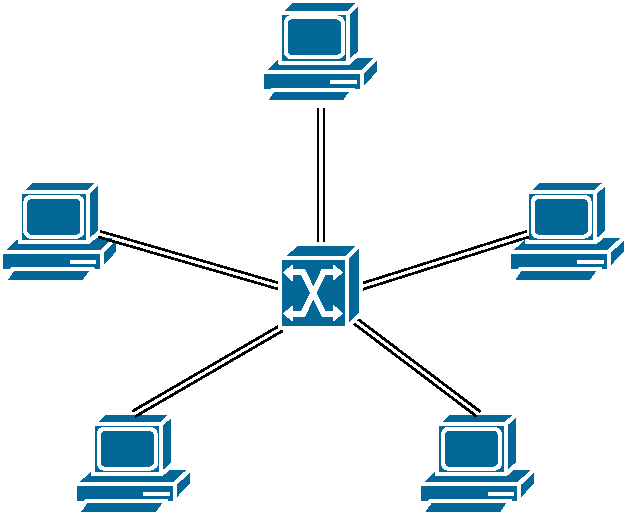
\includegraphics[width=0.2\textwidth]{./figuras/Topologia-Estrela.pdf} % <- formatos PNG, JPG e PDF
	%\caption[Exemplo de topologia em estrela]{Exemplo de topologia conectada em estrela. Percebe-se que todos os equipamentos estão ligados a um nó central, neste caso um \emph{switch}.}
	%\label{fig_topologia_estrela}
%\end{figure}

A topologia em árvore, talvez a mais recorrente em redes de computadores, é assim chamada pois pode ser reconhecida pelo seu aspecto onde o nó central representa a base da árvore e os diversos \emph{hosts} representam suas folhas (normalmente representada como uma árvore invertida). Basicamente trata-se de uma estrutura hierárquica de conexão entre várias redes e/ou sub-redes. A Figura \ref{fig_topologia_multiplo_arvore} ilustra esse tipo de topologia. Percebe-se que a topologia assemelha-se à interconexão de várias sub-redes através de equipamentos dedicados.

%\begin{figure}[!htb]
	%\centering
	%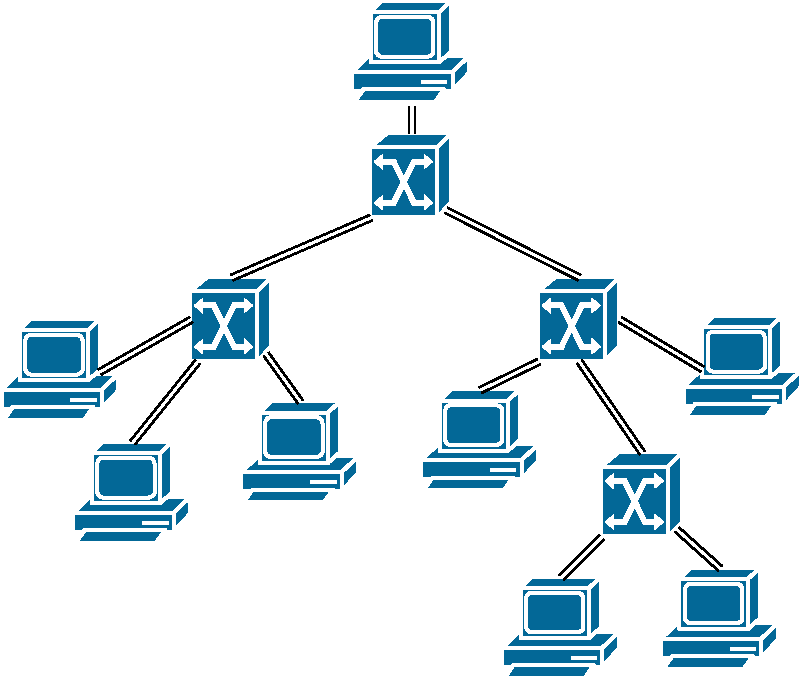
\includegraphics[width=0.2\textwidth]{./figuras/Topologia-Arvore.pdf} % <- formatos PNG, JPG e PDF
	%\caption[Exemplo de topologia em árvore]{Exemplo de topologia conectada em árvore. Percebe-se que a topologia assemelha-se à interconexão de várias sub-redes através de equipamentos dedicados.}
	%\label{fig_topologia_arvore}
%\end{figure}

A topologia em malha ou \emph{mesh} por sua vez, é caracterizada pela criação de uma rede grandemente (podendo chegar a ser plenamente) interconectada, formando diversos caminhos redundantes para a interligação entre a origem e o destino das mensagens. Fato que confere a este tipo de rede um elevado grau de disponibilidade, visto que mesmo em caso de falha de equipamentos ou da infraestrutura a comunicação não é necessariamente comprometida. A Figura \ref{fig_topologia_multiplo_mesh} ilustra uma rede \emph{mesh}. É possível notar que existem diversas rotas redundantes devido aos vários links estabelecidos entre os equipamentos da rede.

%\begin{figure}[!htb]
	%\centering
	%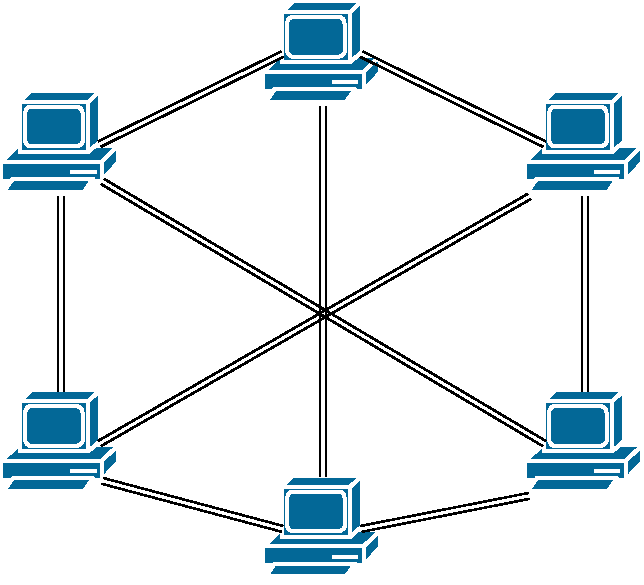
\includegraphics[width=0.2\textwidth]{./figuras/Topologia-Mesh.pdf} % <- formatos PNG, JPG e PDF
	%\caption[Exemplo de topologia em \emph{mesh}]{Exemplo de topologia conectada em \emph{mesh}. Percebe-se existem diversas rotas redundantes devido aos vários links estabelecidos entre os equipamentos da rede.}
	%\label{fig_topologia_mesh}
%\end{figure}

\begin{figure}[t!]
	\centering
	\begin{subfigure}[t]{0.4\textwidth}
		\centering
		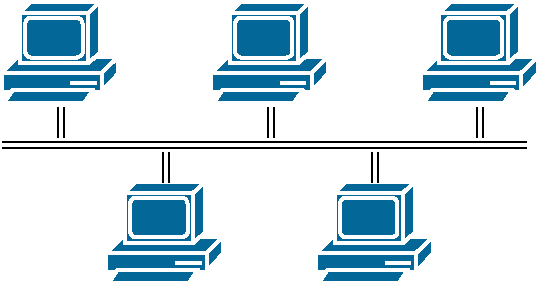
\includegraphics[width=4cm]{./figuras/Topologia-Barramento.pdf} % <- formatos PNG, JPG e PDF
		\caption{Topologia em barramento.}
		\label{fig_topologia_multiplo_barramento}
	\end{subfigure}%
	~
	\begin{subfigure}[t]{0.4\textwidth}
		\centering
		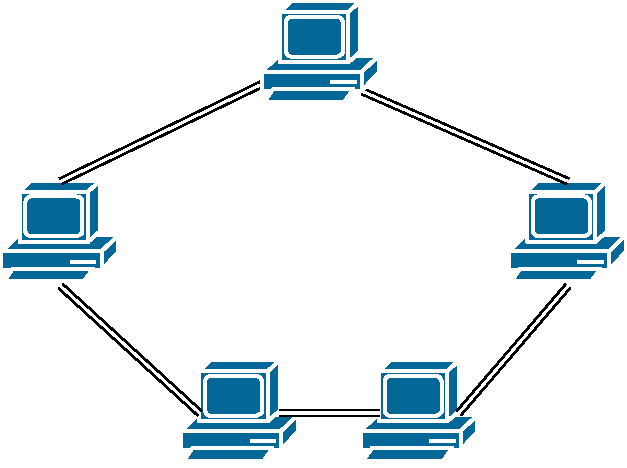
\includegraphics[width=4cm]{./figuras/Topologia-Anel.pdf} % <- formatos PNG, JPG e PDF
	\caption{Topologia em anel.}
	\label{fig_topologia_multiplo_barramento_anel}
	\end{subfigure}
	~
	\begin{subfigure}[t]{0.4\textwidth}
		\centering
		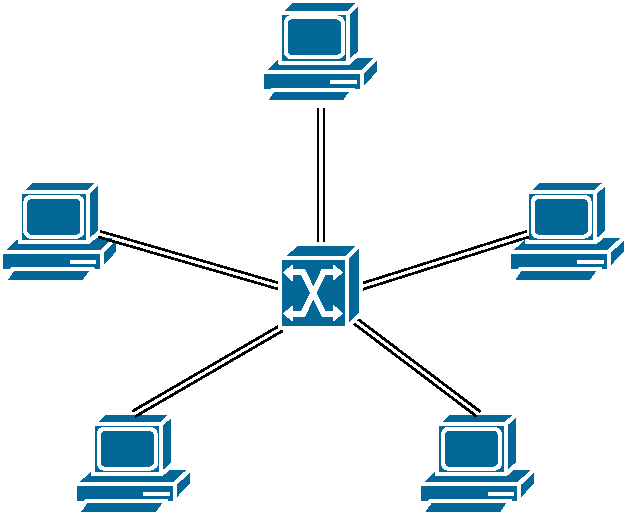
\includegraphics[width=4cm]{./figuras/Topologia-Estrela.pdf} % <- formatos PNG, JPG e PDF
	\caption{Topologia em estrela.}
	\label{fig_topologia_multiplo_estrela}
	\end{subfigure}
	~
	\begin{subfigure}[t]{0.4\textwidth}
		\centering
		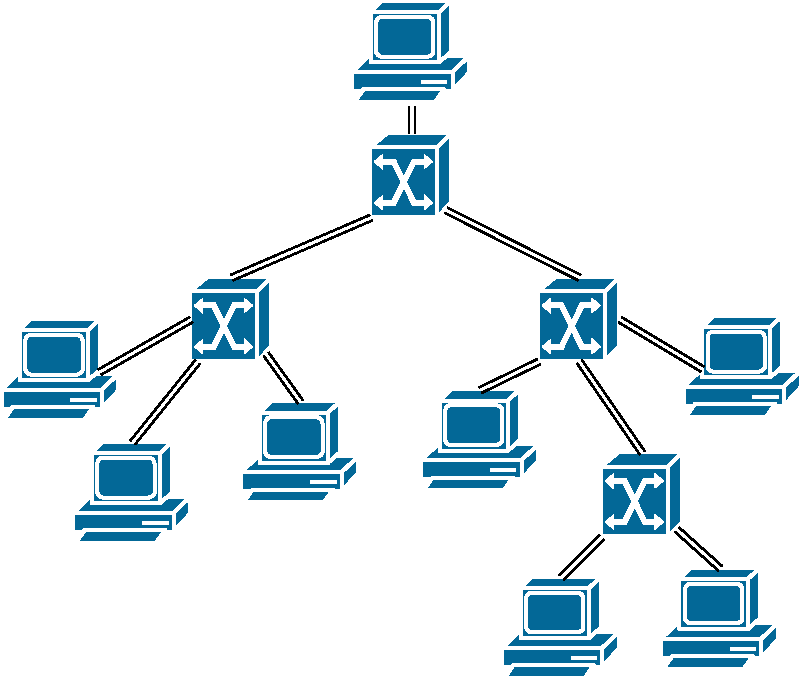
\includegraphics[width=4cm]{./figuras/Topologia-Arvore.pdf} % <- formatos PNG, JPG e PDF
	\caption{Topologia em árvore.}
	\label{fig_topologia_multiplo_arvore}
	\end{subfigure}
	~
	\begin{subfigure}[t]{0.4\textwidth}
		\centering
		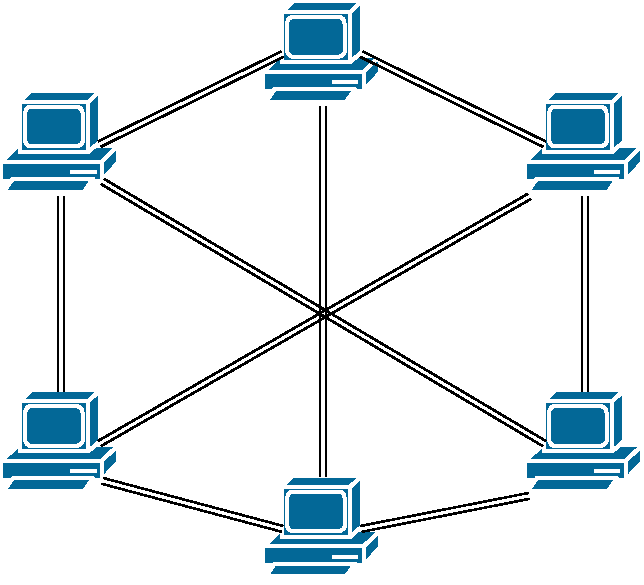
\includegraphics[width=4cm]{./figuras/Topologia-Mesh.pdf} % <- formatos PNG, JPG e PDF
	\caption{Topologia em \emph{mesh}.}
	\label{fig_topologia_multiplo_mesh}
	\end{subfigure}
	\caption{Tipos básicos de topologia}
	\label{fig_topologia_multiplo}
\end{figure}

\subsection{Tecnologia de Transmissão}
A tecnologia de transmissão está diretamente ligada ao meio físico utilizado, que não precisa ser necessariamente construído em cabos metálicos. Podem ser utilizados fibras ópticas, enlaces de micro-ondas, ondas infravermelhas, satélites de comunicação, entre outros \cite{Book-Tanenbaum2003}. 

Além disso, as redes de computadores podem, e comumente são, criadas através da interconexão de redes híbridas, ou seja, diferentes sub-redes criadas com tecnologias de transmissão distintas. Essas redes por sua vez têm diferentes taxas de transmissão e valores típicos de latência e demais parâmetros aos quais todos os pacotes que as atravessarem estarão submetidos \cite{Book-Kurose2013}. Logo, quando é necessário realizar uma comunicação entre \emph{hosts} em redes que utilizam tecnologias de transmissão diferentes é necessária a existência de algum tipo de mecanismo para regulação da velocidade de transferência de informação assim como políticas de garantia de entrega dos dados. Estes mecanismos são algumas das responsabilidades básicas dos protocolos de roteamento como o TCP/IP.

\subsection{Comutadores Ópticos}
A comunicação em redes ópticas é feita através da modulação de sinais luminosos, cada um desses sinais possui uma frequência diferente (usualmente também chamada de cor do sinal) o que implica em diferentes comprimentos de onda (\simbolo{$\lambda$}{comprimento de onda}). Redes complexas e com grande número de $\lambda$s  como as redes ópticas atuais, possuem em seus nós centrais equipamentos conhecidos como comutadores ópticos, também chamados de \sigla{OXC}{Optical Cross Connect}. OXCs podem realizar roteamento interno de sinais de maneira puramente óptica, puramente elétrica ou até mesmo híbrida\cite{Book-Ramaswami2010}. Existem basicamente três diferentes classificações de equipamentos OXC, os opacos, os transparentes e os translúcidos.
%Usar Optical Networks pagina 488
OXC opacos são assim chamados por impedirem a passagem direta da luz, ou seja, o roteamento que esse tipo de equipamento oferece é realizado no domínio elétrico. Para isso todos os sinais que entram no equipamento são convertido em sinais elétricos e enviados a um \emph{switch} ou processador eletrônico que fará o devido roteamento, para que então esses sinais sejam novamente convertidos em sinais ópticos através da utilização de \emph{transceivers} e lasers. Este tipo de equipamento é amplamente empregado em redes ópticas atuais e são muitas vezes conhecidos como \sigla{OEO}{Optical-Electrical-Optical} ou Óptico-Elétrico-Óptico em tradução livre.

Equipamentos OXC opacos possuem o inconveniente de que a circuitaria eletrônica utilizada acaba por limitar a banda do sinal. Existem diversas razões para esta limitação sendo as principais delas as conversões de meio necessárias e o poder de processamento do próprio equipamento. Apesar disso, a grande vantagem deste tipo de equipamento reside no custo benefício, já que ele possibilita a regeneração do sinal óptico a cada nó da rede, visto que o sinal precisa ser recriado, e o controle e obtenção de métricas relativas à comunicação transportada por ele.  

OXC transparentes por sua vez, são assim chamados por não interromperem o sinal de luz que os transpassa. Esse tipo de equipamento tem a capacidade de realizar a separação dos comprimentos de onda de luz e seu devido encaminhamento ou roteamento para a interface desejada. 

Em linhas gerais, a luz que chega ao equipamento (composta por diferentes $\lambda$s) é demultiplexada de acordo com a sua cor ou $\lambda$, direcionada para a saída desejada e unida aos demais sinais luminosos da respectiva saída através de um multiplexador, para então serem enviados através de uma fibra óptica. 

Percebe-se que este tipo de equipamento faz a divisão e roteamento de luz em grande parte de maneira passiva, alterando o menos possível os sinais que por ele transitam (normalmente o efeito mais significativo sobre o sinal está relacionado à potência e separação de $\lambda$s do mesmo), logo o sinal não é demodulado/interpretado impedindo a obtenção de métricas de qualidade ou controle sobre a comunicação. Além disso, estes equipamentos costumam ter sua performance grandemente atrelada a dispositivos sensíveis, como filtros internos, o que acarreta em um custo final elevado. A Figura \ref{fig_oxc_optico} contém o diagrama básico de um OXC transparente. Razões estas que impedem sua ampla utilização em redes ópticas de grande porte.

\begin{figure}[!htb]
	\centering
	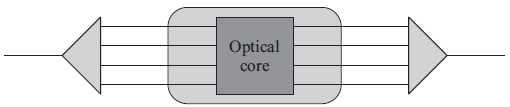
\includegraphics[width=0.5\textwidth]{./figuras/OXC-Optico.png} % <- formatos PNG, JPG e PDF
	\caption[Exemplo básico de OXC óptico]{Exemplo básico de um equipamento OXC transparente. Percebe-se que o sinal de entrada é apenas repassado à respectiva saída sem nenhuma outra intervenção.}
	\fonte{\cite{Book-Ramaswami2010}}
	\label{fig_oxc_optico}
\end{figure}

Por fim, um OXC translúcido traduz-se em um equipamento que representa um compromisso entre os dois tipos anteriores. Ou seja, um equipamento de roteamento em redes ópticas que tem a capacidade de processamento de pacotes e de chaveamento de luz. Este tipo de equipamento, apesar de não ser comumente encontrado, é o foco do presente trabalho.

A proposta que será detalhadamente descrita no Capítulo \ref{capitulo_proposta} pode ser usada para transformar um equipamento óptico seja qual for em um equipamento similar a um OXC translúcido através da utilização de chaveadores ópticos ou \emph{switches} ópticos.

Chaveadores ópticos são componentes capazes de desviar um feixe luminoso através da utilização de um prisma refletor. A Figura \ref{fig_chaveador_optico} mostra o diagrama interno simplificado de um chaveador óptico, percebe-se que seu funcionamento é análogo ao de um relé elétrico.

\begin{figure}[!htb]
	\centering
	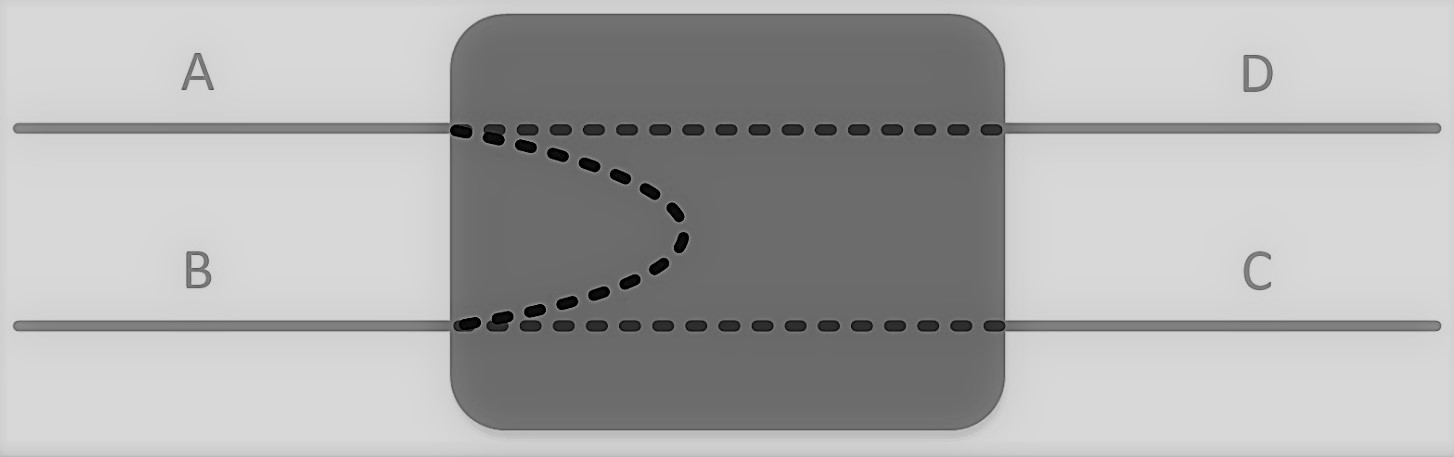
\includegraphics[width=0.5\textwidth]{./figuras/Switch_optico.jpg} % <- formatos PNG, JPG e PDF
	\caption[Exemplo básico chaveador óptico]{Diagrama interno simplificado de um chaveador óptico. Em um estado este componente transmite bidirecionalmente a luz da interface A para D e B para C, quando acionado ele transmite bidirecionalmente a luz da interface A para B.}
	\fonte{Adaptado de \cite{Accelink2014}}
	\label{fig_chaveador_optico}
\end{figure}

A utilização de um chaveador óptico em conjunto com um equipamento OEO pode conferir-lhe a capacidade de desviar sinais ópticos caso necessário, surgindo assim um equipamento de roteamento que pode ser classificado como sendo um OXC 
\section{Protocolos de Roteamento}
\label{cap_protocolos_de_roteamento}
Este capítulo destina-se à discussão de alguns dos protocolos de roteamento recorrentemente utilizados no cenário descrito.

\subsection{Definição de Protocolo}
Assim como no mecanismo formal de troca de informações entre humanos um protocolo de comunicação é o que estabelece as regras básicas para troca de dados entre máquinas. Segundo \cite{Book-Kurose2013} um procolo de comunicação define o formato e a ordem das mensagens trocadas entre duas ou mais entidades, assim como as ações necessárias para que esses dados sejam corretamente recebidos/enviados. A Figura \ref{fig_explicacao_protocolo} exemplifica este paralelo.

\begin{figure}[!htb]
	\centering
	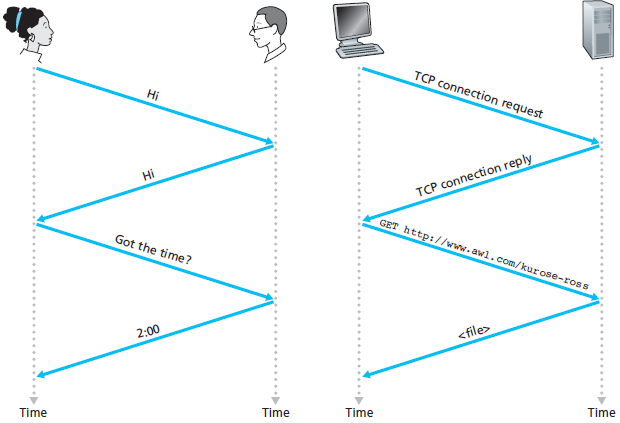
\includegraphics[width=0.5\textwidth]{./figuras/Explicacao-Protocolo.png} % <- formatos PNG, JPG e PDF
	\caption[Exemplo de Protocolo de Comunicação]{Exemplo de Protocolo de Comunicação, o paralelo entre o mecanismo de comuniacação entre humanos e um protocolo de comunicação entre máquinas exemplifica a definição de ``protocolo''.}
	\fonte{\cite{Book-Kurose2013}}
	\label{fig_explicacao_protocolo}
\end{figure}

Um protocolo de comunicação pode ser implementado em software, hardware ou em uma combinação de ambos. De maneira geral, eles são convenientemente separados em camadas ou \emph{layers}, que por sua vez oferecem ``serviços'' aos \emph{layers} superiores \cite{Book-Kurose2013}. Esses \emph{layers} são normalmente baseados em um modelo conhecido como Modelo de Referencia \sigla{OSI}{\emph{Open Systems Interconnection}} convenientemente representado na Figura \ref{fig_modelo_OSI}. Essa modularidade é extremamente útil visto que fornece um nível de abstração interessante aos protocolos, possibilitando por exemplo que o mesmo protocolo possa ser utilizado independentemente do meio físico em questão.

\begin{figure}[!htb]
	\centering
	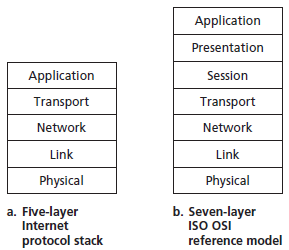
\includegraphics[width=0.4\textwidth]{./figuras/Modelo-OSI.png} % <- formatos PNG, JPG e PDF
	\caption[Modelo OSI]{Comparação entre o Modelo de Referência OSI e a pilha de protocolos de Internet.}
	\fonte{\cite{Book-Kurose2013}}
	\label{fig_modelo_OSI}
\end{figure}

\subsection{Descrever protocolos comuns???}


%---------- Terceiro Capitulo ----------
\chapter{Proposta}
\label{capitulo_proposta}
Os atrasos existentes em equipamentos elétricos utilizados em redes ópticas têm diversas origens, como o processamento dos dados (intrinsecamente relacionado ao poder de processamento do equipamento) e as conversões de meio necessárias, sendo que para cada equipamento pode-se considerar pelo menos duas dessas conversões (óptica-elétrica-óptica). 

Logo, todas as vezes que um pacote trafega em uma rede óptica acaba sofrendo atrasos, que são traduzidos em forma de latência, em cada um dos nós participantes do circuito. Estes atrasos devem ser somados a fim de determinar a latência total de um enlace. A Figura \ref{fig_latency_link} mostra a acúmulo da latência através de um enlace óptico entre dois pontos. 

\begin{figure} [!htb]% normalmente utilizar [!t]
	\centering
	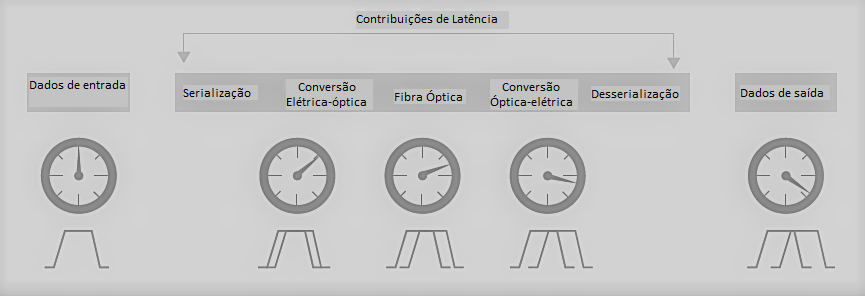
\includegraphics[width=1\textwidth]{./figuras/latency-link.png}
	\caption[Latência de Link]{Latência em comunicação entre dois pontos utilizando link óptico. Os principais pontos de inserção de latência na comunicação são resultantes dos processos de conversão elétrica-óptica, transmissão de dados, conversão óptica-elétrica e disponibilização dos dados no destino (desserialização e processamento).}
	\fonte{\cite{Art-Coffe2017}}
	\label{fig_latency_link}
\end{figure}

Logo, a proposta apresentada neste artigo, denominada de \sigla{BSN}{\emph{``Bypass Seletivo de Nós''}} \emph{``Bypass Seletivo de Nós''}, ocupa um lugar intermediário entre os equipamentos puramente ópticos e os ópticos/elétricos. Conforme descrito na seção \ref{cap_protocolos_de_roteamento} um protocolo de roteamento é responsável pelo tratamento e pela dinâmica das mensagens e dados trocados entre os dispositivos participantes da comunicação. Como dinâmica pode-se citar o cálculo de rotas a serem utilizadas e, desta forma pode-se configurar o BSN como um protocolo especificamente desenvolvido para otimização de latência em redes ópticas através da utilização de chaveadores ópticos em pontos estratégicos da rede, ou seja, através da manipulação do \emph{layer} físico da rede. Dessa forma equipamentos em posições específicas da rede podem ser desviados sem a necessidade de nenhuma conversão de meio ou mesmo processamento, resultando na mínima inserção de latência possível. 

O BSN opera de maneira completamente desagregada do protocolo de roteamento utilizado na rede em questão. Ele pode ser utilizado em qualquer rede que contenha multi-caminhos ou redundâncias de maneira a possibilitar a criação de novas topologias a partir da reorganização das ligações físicas. Para tanto, é necessário que a rede em questão possa ser representada por um grafo simples, ou seja, um grafo que não possui arestas paralelas ou pontas coincidentes (laços) conforme anteriormente descrito em \ref{chap_grafos}.

Os pontos da rede de acionamento do chaveador óptico podem ser escolhidos em ramos de um grafo com muitos vértices (\emph{hops}) ou podem ser planejados para o estabelecimento de rotas específicas para comunicação com pontos críticos do sistema, estabelecendo um \sigla{SLA}{\emph{Service Level Agreement}} em \emph{layer} físico.

Através da utilização do BSN é possível reduzir o grafo da rede possibilitando uma nova configuração de conexões inexistente na rede original e consequentemente uma nova variedade de rotas possíveis. Cada vez que o BSN ativa um \emph{bypass}, as duas arestas envolvidas são unificadas evitando o vértice das mesmas, criando assim um novo grafo com uma distância entre os dois vértices finais de um vértice a menos, como representado na Figura \ref{fig-bypass-exemplo}. Dessa forma, em caso de falha ou mudança de SLA, a topologia física pode ser alterada automaticamente.

\begin{figure}[t!]
	\centering
	\begin{subfigure}[t]{0.4\textwidth}
		\centering
		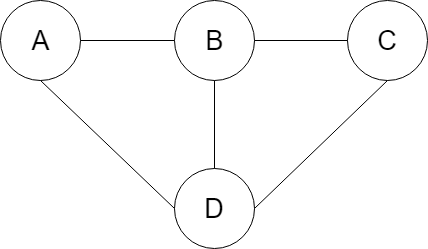
\includegraphics[width=4cm]{./figuras/Bypass-exemplo-A.png} % <- formatos PNG, JPG e PDF
		\caption{Chaveador óptico desativado}
		\label{fig_bypass_exemplo_A}
	\end{subfigure}%
	~
	\begin{subfigure}[t]{0.4\textwidth}
		\centering
		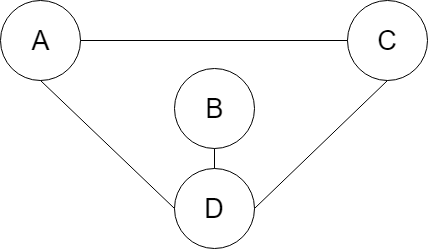
\includegraphics[width=4cm]{./figuras/Bypass-exemplo-B.png} % <- formatos PNG, JPG e PDF
	\caption{Chaveador óptico ativado}
	\label{fig_bypass_exemplo_B}
	\end{subfigure}
	\caption[Exemplo de atuação de \emph{by-pass} óptico]{Efeito da utilização do chaveador ótico em uma rede de comunicação. Em \ref{fig_bypass_exemplo_A} pode-se ver a rede original contendo dois saltos entre os vértices A e C. Em \ref{fig_bypass_exemplo_B} após o acionamento do dispositivo no vértice B pode-se ver e existência de apenas um salto entre os vértices A e C}
	\label{fig-bypass-exemplo}
\end{figure}

\section{BSN}
Esta seção descreve o funcionamento da proposta através de um exemplo simplificado, discorre sobre a implementação do algoritmo utilizado para criação do BSN assim como sobre a ferramenta criada para simulações e criação dos dados utilizados no presente estudo.

\subsection{Funcionamento do BSN}
Para exemplificar o funcionamento do BSN foi gerada a rede da Figura \ref{BSN-example-network}. Essa rede foi gerada pelo software desenvolvido para avaliação do BSN, posteriormente descrito de maneira detalhada na Seção \ref{implementacao}. Como pode-ser notar essa rede é representada por um grafo simples com valência igual a 3, e pode ser classificada de acordo com o exposto na Seção \ref{redes-de-computadores} com sendo uma rede \emph{mesh}. 

O grafo da Figura \ref{BSN-example-network} foi submetido ao software de simulação para cálculo dos caminhos ótimos para todos os vértices à partir do vértice origem (arbitrariamente escolhido como sendo o 1) e a Figura \ref{BSN-example-network-tree} mostra o resultado desta operação. Esta figura representa os caminhos ótimos para, saindo do vértice raiz, alcançar todos os demais vértices. Deste modo, grafo da Figura \ref{BSN-example-network-tree} representa o melhor caso possível em termos de profundidade de rede.

Após as melhores rotas terem sido descobertas conforme descrito, a rede da Figura \ref{BSN-example-network} foi submetida ao software de simulação para a execução do BSN. Como resultado decidiu-se pelo acionamento do chaveador óptico no vértice 7, interligando o vértice 1 diretamente ao 4 gerando um novo grafo da rede conforme representado na Figura \ref{BSN-example-opt-switch}. Este grafo, quando submetido ao cálculo dos caminhos ótimos, assim como realizado com a rede original, resulta no grafo da Figura \ref{BSN-example-rede-otimizada}, onde pode-se notar a diminuição da profundidade em comparação com aquele mostrado na Figura \ref{BSN-example-network-tree}.

\begin{figure}[t!]
	\centering
	\begin{subfigure}[t]{0.4\textwidth}
		\centering
		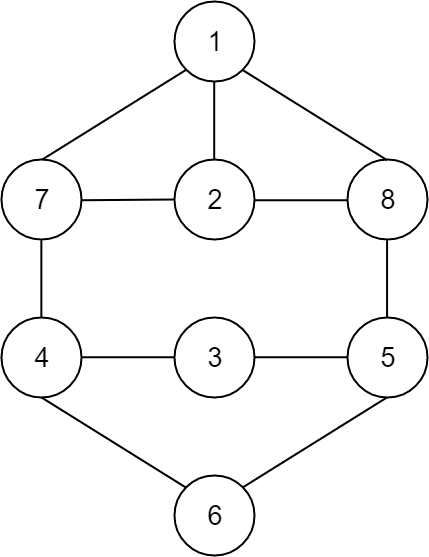
\includegraphics[width=4cm]{./figuras/BSN-ex-network-generation.png} % <- formatos PNG, JPG e PDF
		\caption{Rede gerada}
		\label{BSN-example-network}
	\end{subfigure}%
	~
	\begin{subfigure}[t]{0.4\textwidth}
		\centering
		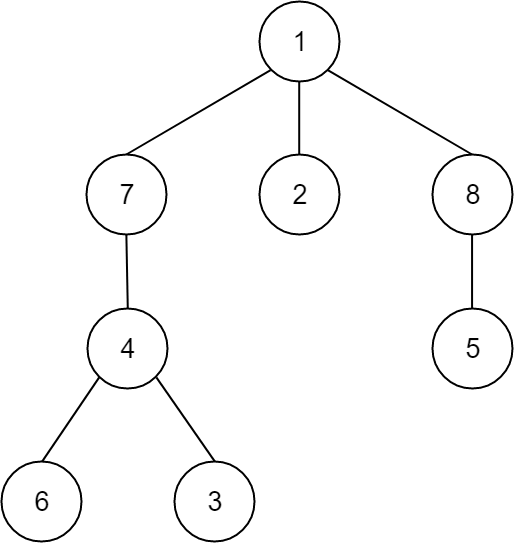
\includegraphics[width=4cm]{./figuras/BSN-ex-network-generation-tree.png} % <- formatos PNG, JPG e PDF
	\caption{Árvore da Rede}
	\label{BSN-example-network-tree}
	\end{subfigure}
	~
	\begin{subfigure}[t]{0.4\textwidth}
		\centering
		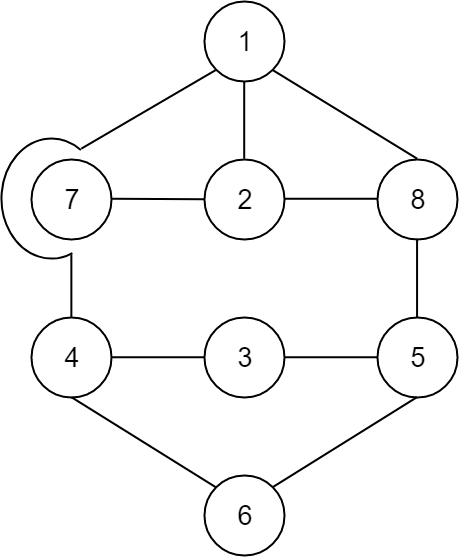
\includegraphics[width=4cm]{./figuras/BSN-ex-bypass.png} % <- formatos PNG, JPG e PDF
	\caption{Chaveador óptico ativado}
	\label{BSN-example-opt-switch}
	\end{subfigure}
	~
	\begin{subfigure}[t]{0.4\textwidth}
		\centering
		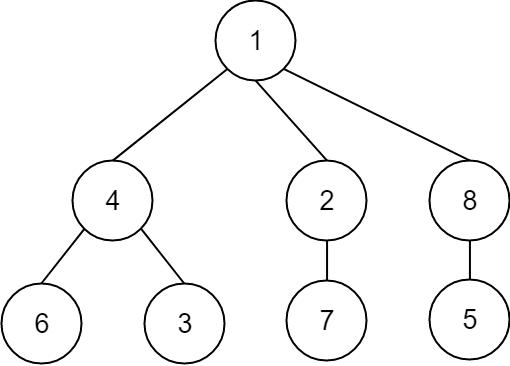
\includegraphics[width=4cm]{./figuras/BSN-ex-network-final.png} % <- formatos PNG, JPG e PDF
	\caption{Rede resultante}
	\label{BSN-example-rede-otimizada}
	\end{subfigure}
	\caption[Exemplo de funcionamento do BSN]{Exemplo de funcionamento do protocolo BSN. Percebe-se que o BSN consegue reduzir a profundidade de uma rede gerando uma nova possibilidade de conexões através da manipulação da camada física da mesma.}
	\label{fig-bsn-exemplo}
\end{figure}

Este exemplo ilustra, em uma rede de apenas 8 nós, o funcionamento do protocolo proposto (BSN). É possível notar que a profundidade da rede, ligada à latência da comunicação, é reduzida impactando na redução de latência para a comunicação entre os nós envolvidos.

\subsection{Implementação}
\label{implementacao}
O método de redução do grafo de rede utilizado pelo BSN é descrito sucintamente em alto nível através do fluxograma apresentado na Figura \ref{fig_bsn_flow}, também apresentado de maneira pouco mais detalhada no pseudocódigo representado no Algoritmo \ref{pseudocode_bsn}. O BSN utiliza vários conceitos de otimização simultâneos. A ideia básica é a utilização de um algoritmo genético para a criação de diferentes combinações de estado dos chaveadores ópticos na rede (de acordo com as premissas de projeto a serem adotadas). Dessa forma, cada uma das combinações geradas pelo algoritmo genético acaba por gerar uma nova topologia de conexões físicas, que são por sua vez otimizadas buscando obter a rede menos profunda possível. 

Esta busca compreende, em essência, a escolha de quais arestas do grafo serão utilizadas para estabelecer a comunicação entre os nós e quais não serão utilizadas. Dessa forma, para o passo representado na linha \ref{bsn:fitness_line} do Algoritmo \ref{pseudocode_bsn} (busca local), que representa exatamente este passo do código, pode ser utilizado qualquer algoritmo conhecido. Daí vem o fato de o BSN ter a capacidade de ser utilizado com qualquer protocolo padrão de otimização de rede como o STP por exemplo. O presente documento utiliza para este passo uma busca de custo uniforme, garantindo assim a obtenção do valor ótimo de \emph{fitness}, que neste código está relacionado ao custo total da rede. Ou seja, o algoritmo de custo uniforme irá resultar na melhor rede possível para o grafo em questão já que este tipo de busca é exaustiva e explora todas as combinações possíveis para então selecionar a melhor delas.

\begin{figure} [t]% normalmente utilizar [!t]
	\centering
	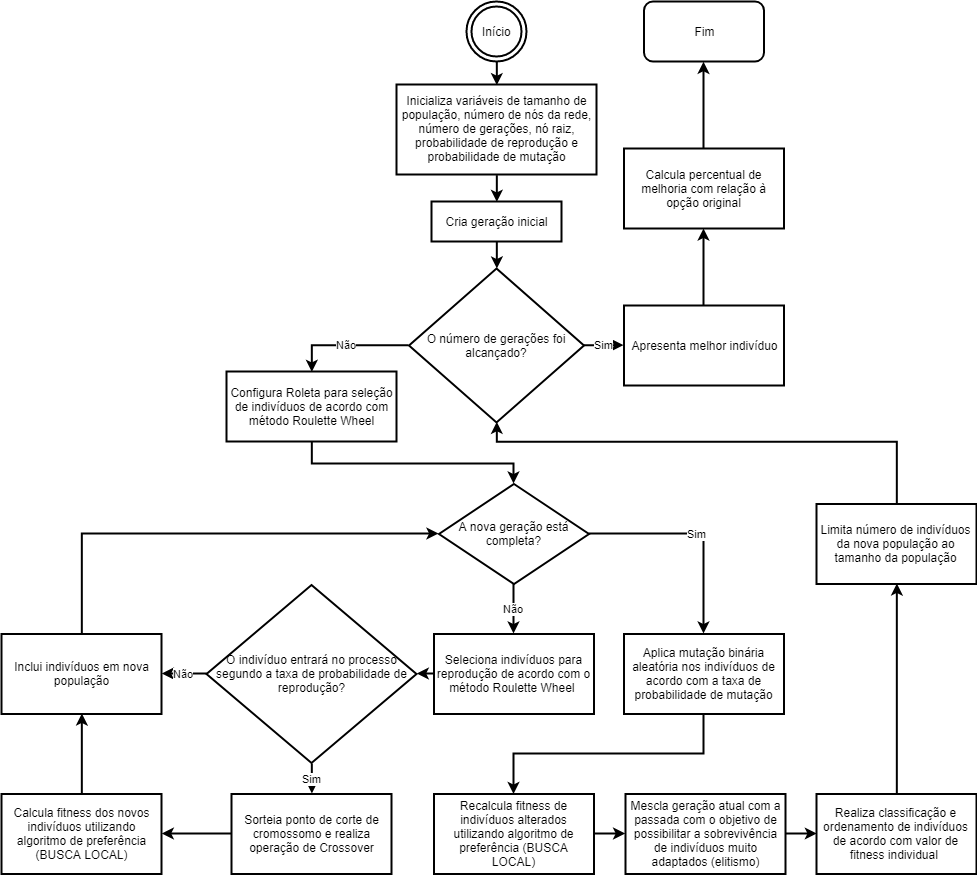
\includegraphics[width=1\textwidth]{./figuras/BSN-Flow.png}
	\caption[Fluxograma do BSN]{Representação de fluxograma em alto nível do funcionamento do BSN}
	\label{fig_bsn_flow}
\end{figure}

\begin{algorithm} [h]
\caption{ - Algoritmo básico do BSN}
\begin{algorithmic}[1]
\State $popsize\gets \textit{tamanho da populacao}$
\State $gennumb\gets \textit{numero de geracoes}$\\
\State PopList[] = new List[popsize]\Comment{Variável para alocação da geração atual}
\State $i\gets 0$
\While {$ i< popsize $}
\State Individuo = CriaIndividuo()\Comment{Cria a uma configuração de rede}
\State CalculaFit(Individuo)\label{bsn:fitness_line}\Comment{Realiza busca local na instância de rede}
\State PopList.Add(Individuo)\Comment{Adiciona a instância de rede à lista}
\State PopList.ClassifcaIndividuos()\Comment{Organiza a população atual de acordo com o Fitness individual}
\EndWhile\Comment{População inicial criada}\\
\State $j\gets 1$
\While {$ j< gennumb $}\Comment{Roda algoritmo genético}
\State ParentsList[] = new List[]\Comment{Variável para alocação de indivíduos ``pais''}
\State NewList[] = new List[popsize]\Comment{Variável para alocação de próxima geração}
\State ParentsList = SelecionaIndividuos(PopList)\Comment{Seleciona os indivíduos da geração atual que serão utilizados para criação da geração seguinte}
\State NewList = CrossOver(ParentsList)\Comment{Cruza os indivíduos selecionados}
\State Mutation(NewList)\Comment{Aplica algoritmo de mutação de genes na nova população}
\State PopList = MesclaGen(NewList, PopList)\Comment{Realiza elitismo de indivíduos}
\State PopList.ClassifcaIndividuos()\Comment{Organiza a população atual de acordo com o Fitness individual}
\EndWhile\\
\State\Return PopList.Individuo(0)\Comment{Retorna melhor instância de rede}
\end{algorithmic}
\label{pseudocode_bsn}
\end{algorithm}

\subsubsection{Custo da rede}
\label{subsection-custo-da-rede}
O custo da rede é definido como a soma de todos os custos individuais (número de saltos) para comunicação em cada um dos \emph{links} da rede. Logo, utilizando a rede de exemplo representada na Figura \ref{BSN-example-network-tree} tem-se o mostrado na Tabela \ref{tab-custo-rede-BSN-example-network-tree} como sendo os custos individuais para comunicação entre o nó origem e os demais assim como o custo total da rede. Em contrapartida, ao utilizar a rede representada na Figura \ref{BSN-example-rede-otimizada}, que foi otimizada através da utilização do BSN, tem-se como resultado para os custos individuais e custo total o representado na Tabela \ref{tab-custo-rede-bsn-otimizada}.

A partir da comparação dos dados apresentados na Tabela \ref{tab_calc_custo} nota-se que o custo total da rede foi otimizado em aproximadamente 15,4\% (o que por si só já representa um grande ganho) mas, além disso, ao comparar o custo de cada um dos nós de maneira individual pode-se notar que para os destinos 3 e 6 foi alcançado 33,33\% de melhoria e para os destinos 4 e 7 foi alcançado 50\% de melhoria.

Assim fica claro o BSN não apenas minimiza o custo ou latência da rede como um todo mas apresenta, em especial, um ótimo resultado ao avaliar-se o custo de uma rota em específico. Desta forma o protocolo proposto pode ser extremamente útil no estabelecimento de políticas de \sigla{QoS}{\emph{Quality of Service}} em layer físico, sendo esta uma aplicação jamais explorada anteriormente.

\setcounter{table}{1} \renewcommand{\thetable}{\arabic{table}}
\begin{table}[t!]
	\centering
	\begin{subfigure}[t]{0.4\textwidth}
		\centering
		%\begin{table}[]
			\begin{tabular}{llllll}
			\hline
			\multicolumn{1}{|l|}{\textbf{Nó destino}} & \multicolumn{4}{c}{\textbf{Caminho}} & \multicolumn{1}{c|}{\textbf{Custo}} \\ \hline
			\multicolumn{1}{|l|}{\textbf{2:}} & 1 & 2 &  & \multicolumn{1}{l|}{} & \multicolumn{1}{l|}{1} \\ \hline
			\multicolumn{1}{|l|}{\textbf{3:}} & 1 & 7 & 4 & \multicolumn{1}{l|}{3} & \multicolumn{1}{l|}{3} \\ \hline
			\multicolumn{1}{|l|}{\textbf{4:}} & 1 & 7 & 4 & \multicolumn{1}{l|}{} & \multicolumn{1}{l|}{2} \\ \hline
			\multicolumn{1}{|l|}{\textbf{5:}} & 1 & 8 & 5 & \multicolumn{1}{l|}{} & \multicolumn{1}{l|}{2} \\ \hline
			\multicolumn{1}{|l|}{\textbf{6:}} & 1 & 7 & 4 & \multicolumn{1}{l|}{6} & \multicolumn{1}{l|}{3} \\ \hline
			\multicolumn{1}{|l|}{\textbf{7:}} & 1 & 7 &  & \multicolumn{1}{l|}{} & \multicolumn{1}{l|}{1} \\ \hline
			\multicolumn{1}{|l|}{\textbf{8:}} & 1 & 8 &  & \multicolumn{1}{l|}{} & \multicolumn{1}{l|}{1} \\ \hline
			 & \multicolumn{4}{l}{\textbf{Custo Total}} & \textbf{13}
			\end{tabular}
		\caption{Calculo de custo - Rede Figura \ref{BSN-example-network-tree}}
		\label{tab-custo-rede-BSN-example-network-tree}
		%\end{table}
	\end{subfigure}%
	~
	\begin{subfigure}[t]{0.4\textwidth}
		\centering
			%\begin{table}[]
			\begin{tabular}{lllll}
			\hline
			\multicolumn{1}{|l|}{\textbf{Nó destino}} & \multicolumn{3}{c}{\textbf{Caminho}} & \multicolumn{1}{c|}{\textbf{Custo}} \\ \hline
			\multicolumn{1}{|l|}{\textbf{2:}} & 1 & 2 & \multicolumn{1}{l|}{} & \multicolumn{1}{l|}{1} \\ \hline
			\multicolumn{1}{|l|}{\textbf{3:}} & 1 & 4 & \multicolumn{1}{l|}{3} & \multicolumn{1}{l|}{2} \\ \hline
			\multicolumn{1}{|l|}{\textbf{4:}} & 1 & 4 & \multicolumn{1}{l|}{} & \multicolumn{1}{l|}{1} \\ \hline
			\multicolumn{1}{|l|}{\textbf{5:}} & 1 & 8 & \multicolumn{1}{l|}{5} & \multicolumn{1}{l|}{2} \\ \hline
			\multicolumn{1}{|l|}{\textbf{6:}} & 1 & 4 & \multicolumn{1}{l|}{6} & \multicolumn{1}{l|}{2} \\ \hline
			\multicolumn{1}{|l|}{\textbf{7:}} & 1 & 2 & \multicolumn{1}{l|}{7} & \multicolumn{1}{l|}{2} \\ \hline
			\multicolumn{1}{|l|}{\textbf{8:}} & 1 & 8 & \multicolumn{1}{l|}{} & \multicolumn{1}{l|}{1} \\ \hline
			 & \multicolumn{3}{l}{\textbf{Custo Total}} & \textbf{11}
			\end{tabular}
	\caption{Calculo de custo - Rede Figura \ref{BSN-example-rede-otimizada}}
	\label{tab-custo-rede-bsn-otimizada}
	%\end{table}
	\end{subfigure}
	\caption[Exemplo de cálculo de custo total em rede]{Exemplificação do cálculo e comparação entre o custo total para duas redes exemplo}
	\label{tab_calc_custo}
\end{table}

\subsubsection{Representação}
Na Computação Evolutiva de maneira geral é comum encontrar termos da biologia para representar estruturas e variáveis, o mesmo acontece no campo dos AGs, como no caso do BSN. No presente documento a relação entre estes termos é dada conforme o mostrado na Tabela \ref{tab-correlacao-bio-comp}.

\begin{table}[ht]
\centering
\begin{tabular}{|l|l|}
\hline
\multicolumn{1}{|c|}{\textbf{Biologia}} & \multicolumn{1}{c|}{\textbf{Computação}} \\ \hline
Cromossomo & Indivíduo \\ \hline
Gene & Caractere \\ \hline
Alelo & Valor do caractere \\ \hline
Lócus & Posição do caractere \\ \hline
Genótipo & Vetor de caracteres representando o indivíduo \\ \hline
Fenótipo & Interpretação do vetor de caracteres \\ \hline
\end{tabular}
\caption[Biologia x BSN]{Correlação entre vocábulos da Biologia e os utilizados no BSN}
\label{tab-correlacao-bio-comp}
\end{table}  

Seguindo estas definições, o BSN cria um conjunto de Cromossomos, denominado de população. Esta população é constituída pelos diversos indivíduos cujos Genótipos estão baseados na rede em questão. Cada um dos Cromossomos é representado como sendo um vetor \emph{booleano} com o número de Genes igual ao número de nós da rede a ser otimizada e onde cada um dos Lócus representa unicamente um nó. Os Alelos por sua vez representam o estado do chaveador ótico no respectivo nó. Em resumo, seguindo esta convenção, pode-se representar a rede mostrada na Figura \ref{BSN-example-opt-switch} através do Cromossomo (ou indivíduo) da Tabela \ref{tab-cromossomo-bsn}.

\begin{table}[ht]
\centering
\begin{tabular}{|l|l|l|l|l|l|l|l|l|}
\hline
\multicolumn{1}{|c|}{\textbf{Nó}} & \multicolumn{1}{c|}{1} & 2 & 3 & 4 & 5 & 6 & 7 & 8 \\ \hline
\textbf{Cromossomo} & 0 & 0 & 0 & 0 & 0 & 0 & 1 & 0 \\ \hline
\end{tabular}
\caption[Cromossomo BSN]{Repesentação da estrutura básica de um cromossomo do BSN}
\label{tab-cromossomo-bsn}
\end{table}

Como pode-se notar cada um dos Lócus do Cromossomo representa um nó da rede, logo tem-se um Cromossomo com 8 Genes visto que a rede tem 8 nós, além disso o Alelo do Lócus 7 é igual a 1, o que pode ser interpretado como a informação de que o chaveador óptico instalado no nó 7 está ligado enquanto os outros estão desligados (Alelos 0). Dessa forma, o Fenótipo deste indivíduo, ou seja, a interpretação deste Cromossomo, indica que o grafo desta rede deve ser representado considerando que o chaveador óptico referente ao nó 7 está acionado e os demais não, como representado na Figura \ref{BSN-example-opt-switch}.

\subsubsection{Função de \emph{Fitness}}
Como em qualquer AG o BSN baseia seu funcionamento na avaliação de uma função de \emph{fitness}, que conforme brevemente descrito na Seção \ref{implementacao} está atrelada ao custo da rede. De maneira geral, o custo total da rede é calculado conforme descrito em \ref{subsection-custo-da-rede}, com a diferença da necessidade de adoção de uma convenção em caso da avaliação de um grafo desconexo.

Basicamente, a utilização do BSN pode gerar redes específicas onde nem todos os nós sejam acessíveis devido ao acionamento do chaveador óptico em posições inadequadas. Em outras palavras, podem existir Genótipos que dêem origem a redes cujos grafos são desconexos como o da Figura \ref{fig_grafo_desconexo}. Neste caso o custo dessa rede, de acordo com o descrito em \ref{subsection-custo-da-rede} seria infinito, visto que o custo unitário para alcançar o(s) vértice(s) não conectado(s) seria infinito. Logo necessita-se de uma convenção para representar este custo visto que ``infinito'' não pode ser representado computacionalmente. Adotou-se que o custo de um link como o descrito é igual a 1000 (mil unidades de custo), dessa forma o custo total da rede deverá seguir a Equação \ref{eq-fitness}. Como consequência o custo da rede deverá conter uma parcela múltipla de 1000 no caso em que existam um ou mais nós sem conexão com o nó origem. 

\setcounter{equation}{0} \renewcommand{\theequation}{\arabic{equation}}
\begin{equation}
\begin{split}
Fitness_{BSN} = \sum_{n=1}^{x}custo_{1}(n) \rightarrow custo_{orig}(dst)=\left\{\begin{matrix}
h.p, \textup{para nó conectado}\\ 1000, \textup{para nó desconectado}
\end{matrix}\right.
\\onde:\\
x=\textup{número de nós}
\\orig=\textup{vértice origem}
\\dst=\textup{vértice destino}
\\h=\textup{número de \emph{hops} entre orig e dst}
\\p=\textup{peso do \emph{hop} em questão (custo do link)}
\end{split}
\label{eq-fitness}
\end{equation}

\subsubsection{\emph{Crossover}}
O processo de \emph{Crossover} é o responsável pela criação de novos indivíduos, também chamados de filhos, que serão constituintes da nova geração. Existem muitos métodos diferentes que podem ser utilizados para esta operação, a Figura \ref{fig_crossover} exemplifica o método de \emph{Crossover} simples já que este foi o escolhido no BSN.

\begin{figure} [!htb]% normalmente utilizar [!t]
	\centering
	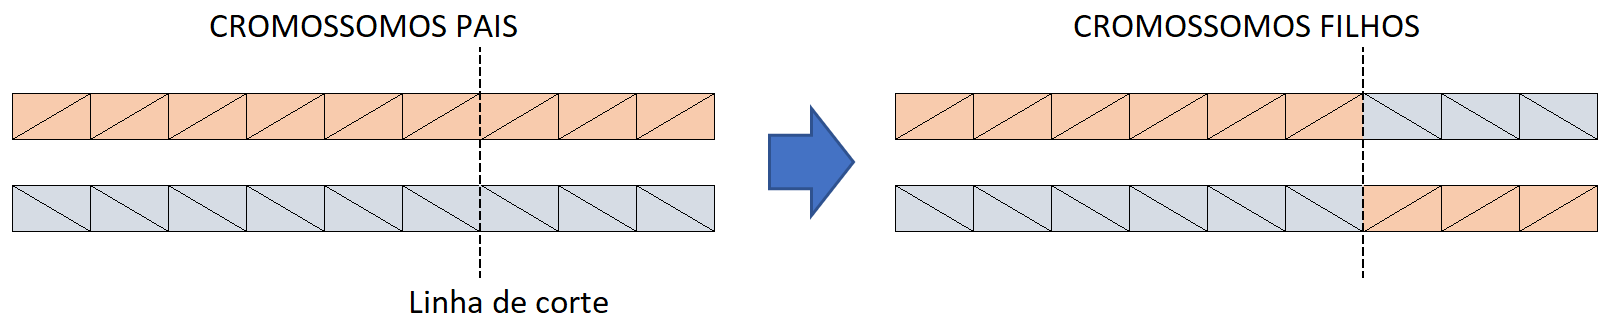
\includegraphics[width=1\textwidth]{./figuras/crossover.png}
	\caption[Exemplo de \emph{Crossover}]{Exemplo de operação de \emph{Crossover} Simples.}
	\label{fig_crossover}
\end{figure}

Como pode-se notar dois cromossomos pais são escolhidos e um ponto de corte é definido de maneira aleatória, os cromossomos são então divididos neste ponto de corte e recriados através da troca de informações entre si. Desta forma os cromossomos filhos são gerados através do compartilhamento de informação genética dos pais, criando um novo indivíduo com um novo valor de \emph{fitness}.

\subsubsection{Seleção}
Paralelamente à Seleção Natural, os AGs utilizam-se de diferentes recursos para selecionar os indivíduos de cada geração mais adaptados ao problema em questão. O BSN utiliza o conceito de \emph{``Roulette Wheel''} \cite{Goldberg1889}. 

Neste tipo de seleção toda a população é avaliada de maneira a criar uma correlação percentual entre o valor de \emph{fitness} de cada um dos indivíduos e sua representatividade perante toda a população. Desse modo pode-se ter um indicativo de quão adaptado cada um deles é com relação a sua geração corrente, e então é possível criar uma distribuição de probabilidades para a escolha de cada um dos mesmos no processo de reprodução.

Seguindo esse critério os pais, que irão fornecer o código genético para a nova geração, deverão potencialmente ser os mais adaptados ao problema em questão aumentando a chance de criar descendentes ainda mais adaptados e, desta forma, acelerando a convergência do algoritmo. A Tabela \ref{tab-selecao} exemplifica este critério de seleção, conforme pode-se ver o indivíduo $\beta$ possui um \emph{fitness} que corresponde a um índice de adaptabilidade ao problema proposto de 43,44\%, logo ele possui 44,33\% de chances de ser escolhido para reprodução enquanto o indivíduo $\alpha$ possui apenas 11,33\% de chance de ser escolhido.

\begin{table}[ht]
\centering
\begin{tabular}{|l|l|l|}
\hline
\multicolumn{1}{|c|}{\textbf{Indivíduo}} & \multicolumn{1}{c|}{\textbf{\emph{Fitness}}} & \textbf{Percentual do Total} \\ \hline
\textbf{$\alpha$} & 34 & 11,33\% \\ \hline
\textbf{$\beta$} & 130 & 43,33\% \\ \hline
\textbf{$\delta$} & 66 & 22\% \\ \hline
\textbf{$\theta$} & 70 & 23,33 \\ \hline
\textbf{Total} & \textbf{300} & \textbf{100\%} \\ \hline
\end{tabular}
\caption[\emph{``Roulette Wheel''}]{Exemplo de aplicação do Método de Seleção \emph{``Roulette Wheel''}}
\label{tab-selecao}
\end{table}

\subsubsection{Dimensão das Populações}
O sucesso de qualquer AG está intrinsecamente relacionado ao tamanho de sua população inicial e das subsequentes gerações. Caso a quantidade de indivíduos em cada uma delas seja muito grande ou muito pequena a evolução dos mesmos pode ser comprometida. Segundo \cite{Goldberg1889} estes parâmetros devem ser estabelecidos empiricamente baseados na disponibilidade dos recursos computacionais utilizados.

Para as simulações do BSN foram utilizadas populações de 500 indivíduos, este valor mostrou-se suficiente para alcançar valores ótimos de custo em várias redes de teste e foi adotado como padrão para as simulações posteriormente descritas.

\subsubsection{Parâmetros Adotados}
\label{parametros}
Para a utilização do BSN, assim como em qualquer AG, alguns parâmetros básicos precisam ser configurados. A Tabela \ref{tab-parametros} mostra os parâmetros utilizados nas simulações do BSN apresentadas na Seção \ref{resultados}, esses parâmetros foram selecionados após exaustivas simulações, tendo por objetivo confirmar que seus valores seriam suficientes para alcançar os resultados desejados.

\begin{table}[ht]
\centering
\begin{tabular}{|l|l|l|l|l|}
\hline
\multicolumn{1}{|c|}{\textbf{\begin{tabular}[c]{@{}c@{}}Tamanho da \\ População\end{tabular}}} & \multicolumn{1}{c|}{\textbf{\begin{tabular}[c]{@{}c@{}}Número de \\ Gerações\end{tabular}}} & \multicolumn{1}{c|}{\textbf{\begin{tabular}[c]{@{}c@{}}Método de escolha\\ de indivíduo para \\ reprodução\end{tabular}}} & \multicolumn{1}{c|}{\textbf{\begin{tabular}[c]{@{}c@{}}Probabilidade de \\ \emph{Crossover}\end{tabular}}} & \multicolumn{1}{c|}{\textbf{\begin{tabular}[c]{@{}c@{}}Probabilidade de \\ Mutação\end{tabular}}} \\ \hline
500 & 50 & \emph{Roulette Wheel} & 94\% & 0,5\% \\ \hline
\end{tabular}
\caption[Parâmetros do BSN]{Parâmetros básicos utilizados no algoritmo do BSN}
\label{tab-parametros}
\end{table}

\subsection{Programa de Simulação}
\label{prog_simulacao}
No presente documento foram consideradas diversas configurações de rede diferentes, para isso foi criado um software de simulação para abastecer o BSN com as informações necessárias para a geração dos resultados apresentados na Seção \ref{resultados}. O funcionamento do programa de simulação criado para esta tarefa é basicamente descrito pelo fluxograma da Figura \ref{fig_prog_simula}.

\begin{figure} [ht]% normalmente utilizar [!t]
	\centering
	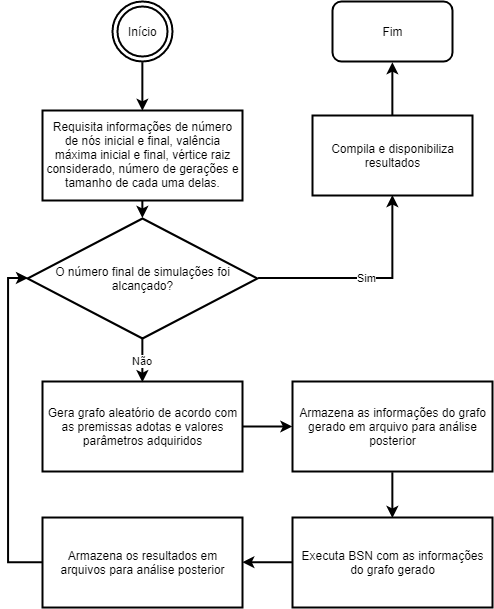
\includegraphics[width=0.6\textwidth]{./figuras/programa-simulacao.png}
	\caption[Fluxograma do Programa de Simulação]{Representação de fluxograma básico do funcionamento do Programa de Simulação criado para o BSN}
	\label{fig_prog_simula}
\end{figure}

Como pode-se perceber o objetivo básico do programa é o de proporcionar a execução do BSN à partir de diferentes configurações de rede de maneira automatizada, entretanto um dos passos representados na Figura \ref{fig_prog_simula} envolve a criação automática de grafos e merece atenção especial.

De acordo com o que foi anteriormente explicado neste documento, o BSN foi originalmente desenvolvido para aplicações em redes SG, principalmente considerando o cenário de distribuição de energia elétrica, logo faz-se necessário a análise de topologia deste tipo de rede de maneira a criar um algoritmo capaz de gerar grafos condizentes com a realidade apresentada nestes cenários.

De acordo com \cite{Conf-Sood2009}, tipicamente existem dois cenários em aplicações SG para distribuição de energia elétrica: um ambiente rural pouco populado ou um ambiente urbano densamente populado e naturalmente conectado em malha. No caso do ambiente rural o desmpenho do BSN, obviamente, pode não apresentar grandes benefícios, visto que as redes de comunicação utilizadas nestes cenários devem dificilmente apresentar alguma redundância. Em contrapartida, as redes presentes nos grandes centros urbanos (densamente populados e naturalmente conectadas em malha) são o objetivo principal da presente proposta.

De maneira geral as redes de distribuição de energia elétrica seguem a topologia da cidade em que são instaladas, ou seja, a disposição das ruas por onde passam. Desta forma fica fácil perceber que as interligações entre equipamentos irão também estar dispostas de acordo com essa premissa. A Figura \ref{fig_esquinas} apresenta algumas das possibilidades mais comuns de disposição de ruas por onde a rede de distribuição deve passar.

\begin{figure}[t!]
	\centering
	\begin{subfigure}[t]{0.4\textwidth}
		\centering
		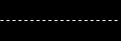
\includegraphics[width=2cm]{./figuras/esquinas1.png} % <- formatos PNG, JPG e PDF
		\caption{Rua sem cruzamento.}
		\label{fig_esquinas1}
	\end{subfigure}%
	~
	\begin{subfigure}[t]{0.4\textwidth}
		\centering
		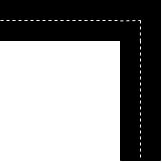
\includegraphics[width=3.5cm]{./figuras/esquinas2.png} % <- formatos PNG, JPG e PDF
	\caption{Esquina comum.}
	\label{fig_esquinas2}
	\end{subfigure}
	~
	\begin{subfigure}[t]{0.4\textwidth}
		\centering
		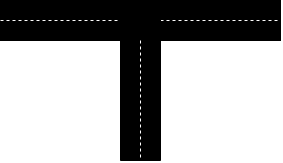
\includegraphics[width=4cm]{./figuras/esquinas3.png} % <- formatos PNG, JPG e PDF
	\caption{Cruzamento em ``T''.}
	\label{fig_esquinas3}
	\end{subfigure}
	~
	\begin{subfigure}[t]{0.4\textwidth}
		\centering
		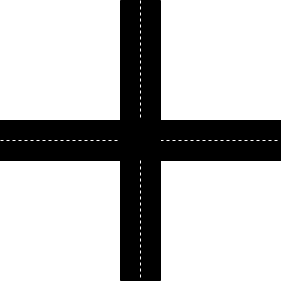
\includegraphics[width=4cm]{./figuras/esquinas4.png} % <- formatos PNG, JPG e PDF
	\caption{Cruzamento clássico.}
	\label{fig_esquinas4}
	\end{subfigure}
	~
	\begin{subfigure}[t]{0.4\textwidth}
		\centering
		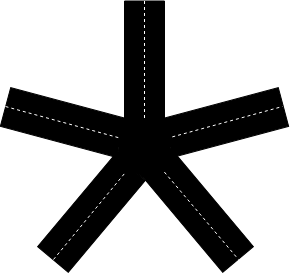
\includegraphics[width=4cm]{./figuras/esquinas5.png} % <- formatos PNG, JPG e PDF
	\caption{Cruzamento em asterisco.}
	\label{fig_esquinas5}
	\end{subfigure}
	\caption{Tipos comuns de cruzamento}
	\label{fig_esquinas}
\end{figure}

As ruas como a representada na Figura \ref{fig_esquinas1} podem conter equipamentos ligados em série ou, eventualmente, equipamentos ``terminais'' que possuam apenas uma conexão com o resto do \emph{grid} como no caso de uma rua sem saída por exemplo. Esse padrão de interligação não muda muito ao considerar ruas como a representada na Figura \ref{fig_esquinas2}. No caso dos cruzamentos como o representado na Figura \ref{fig_esquinas3} fica fácil perceber que podem ser instalados equipamentos com até 3 caminhos redundantes em fibra-óptica, este número aumenta para 4 caminhos redundantes em cruzamentos similares ao da Figura \ref{fig_esquinas4} e 5 para os da Figura \ref{fig_esquinas5}. 

Obviamente a Figura \ref{fig_esquinas} não representa todos os tipos de cruzamentos possíveis e podem ser encontrados outras topologias aqui não mostradas. Entretanto é importante lembrar que para o objetivo específico a que se propõe o presente trabalho, uma redundância de rota pode ser literalmente traduzida como uma redundância de caminho. Ou seja, em um cruzamento como o representado na Figura \ref{fig_esquinas3} não faz sentido utilizar um equipamento com mais de 3 interconexões lógicas visto que neste caso 2 delas deveriam obrigatoriamente chegar ao equipamento utilizando a mesma via de acesso. Isso representaria uma grande falha de projeto, visto que a redundância oferecida por esta conexão extra seria completamente ineficaz no caso de um acidente como o rompimento de um cabo ou apagão. O mesmo princípio se aplica aos demais cruzamentos.

Desta forma, pode-se considerar que para o tipo de rede a que o BSN se propõe, as interconexões entre os equipamentos devem seguir uma distribuição de probabilidades que represente as características físicas da cidade alvo. Com este intuito, foi realizada a análise de algumas redes SG reais brasileiras resultando na distribuição de probabilidades representada na Figura \ref{fig_dist_prob}, esta distribuição foi a utilizada no software de simulação para a geração dos grafos a serem utilizados no presente documento.

\begin{figure} [ht]% normalmente utilizar [!t]
	\centering
	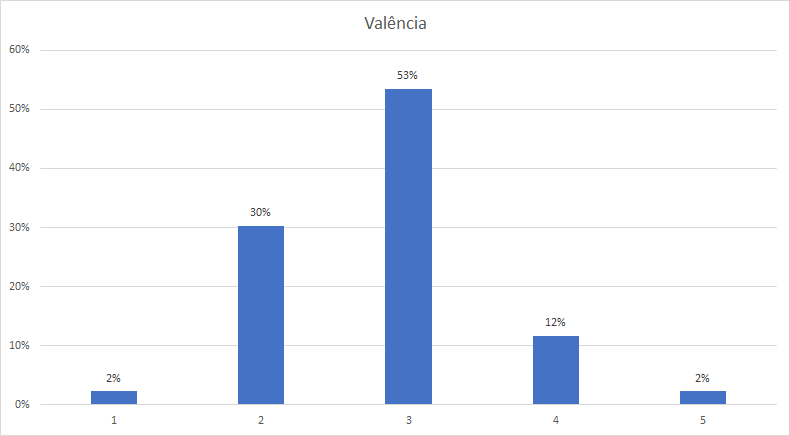
\includegraphics[width=0.85\textwidth]{./figuras/Distribuicao-prob.png}
	\caption[Distribuição de probabilidade]{Distribuição de probabilidade de interligação de equipamentos em redes SG de distribuição de energia elétrica}
	\label{fig_dist_prob}
\end{figure}

Em outras palavras, a geração de grafos utilizadas para a simulação do BSN seguiu a distribuição de probabilidades apresentada na Figura \ref{fig_dist_prob} para determinar a valência máxima e a probabilidade de ocorrência de cada uma delas nos grafos gerados, visando dessa forma representar com maior fidedignidade as redes SG reais.

\section{Resultados}
\label{resultados}
\subsection{Melhoria de custo total}
Para avaliação da performance do BSN foram utilizadas redes criadas aleatoriamente seguindo as premissas de distribuição de probabilidade descritas em \ref{prog_simulacao}. O programa de simulação foi configurado para gerar redes de 5 a 100 nós com passo incremental de 5 unidades, ou seja, foram geradas redes de 5, 10, 15 e assim sucessivamente até 100 nós. Além disso em todas as dimensões de rede foram geradas pelo menos 3 amostras onde uma delas foi limitada a grafos com valência máxima de 3 conexões, a outra com valência máxima de 4 e por fim 5 conexões, tendo por objetivo avaliar a utilização do protocolo proposto diante ao aumento de interconexões máximas em cada nó. É importante notar que o parâmetro alterado em cada um dos casos citados é o de valência máxima, ou seja, apesar de ainda seguir a distribuição de probabilidade de interconexões mostrada em \ref{prog_simulacao}, que representa a topologia física de uma cidade (e que por consequência não é facilmente alterável), simula-se desta forma a utilização de equipamentos com menor número de conexões do que o possível. Fato este recorrente no mundo real devido a limitações de orçamento ou dificuldades de lançamento/instalação de fibras ópticas, ou seja, mesmo em situações onde existe a possibilidade de conexão com vários equipamentos elas não são necessariamente realizadas. Por fim, cada uma das redes foi submetida à execução do BSN configurado com os parâmetros descritos em \ref{parametros}.

A melhoria percentual do custo total da rede foi representada, por questões de facilidade de visualização, para apenas 5 execuções do software de simulação (para cada execução são geradas 20 redes aleatoriamente seguindo as premissas anteriormente expostas) nas Figuras \ref{fig_graph_bsn_val3} a \ref{fig_graph_bsn_val5}.

%\begin{figure}[t!]
	%\centering
	%\begin{subfigure}[t]{0.45\textwidth}
		%\centering
		%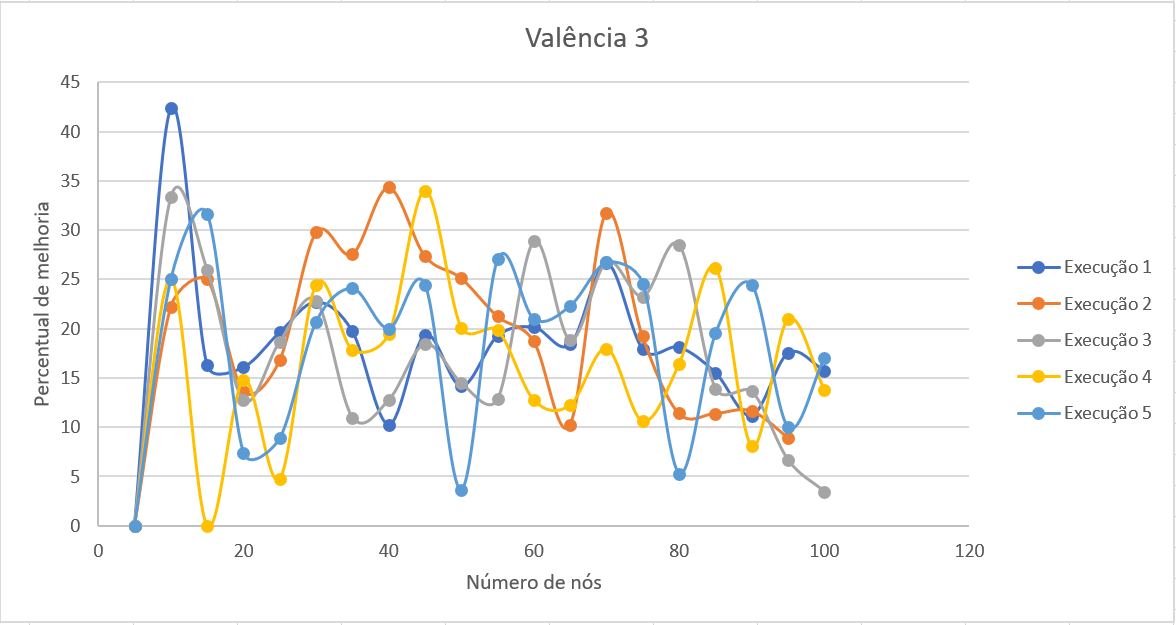
\includegraphics[width=8cm]{./figuras/BSN-valencia3-5exec-grafico.png} % <- formatos PNG, JPG e PDF
		%\caption{Valência máxima 3.}
		%\label{fig_graph_bsn_val3}
	%\end{subfigure}%
	%~
	%\begin{subfigure}[t]{0.45\textwidth}
		%\centering
		%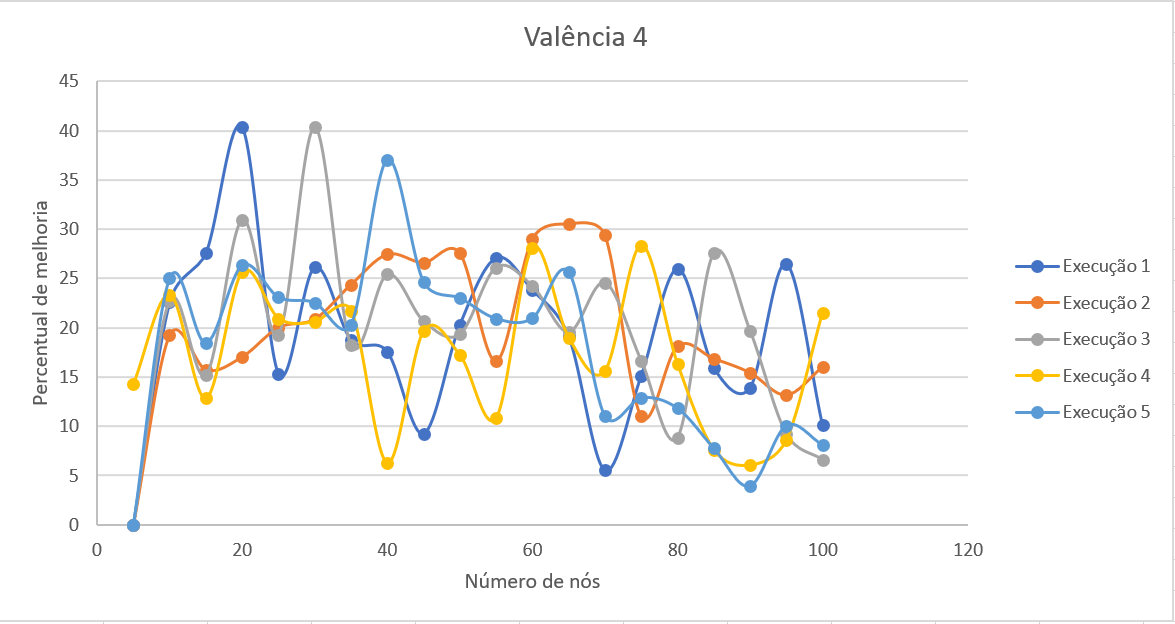
\includegraphics[width=8cm]{./figuras/BSN-valencia4-5exec-grafico.png} % <- formatos PNG, JPG e PDF
	%\caption{Valência máxima 4.}
	%\label{fig_graph_bsn_val4}
	%\end{subfigure}
	%~
	%\begin{subfigure}[t]{0.45\textwidth}
		%\centering
		%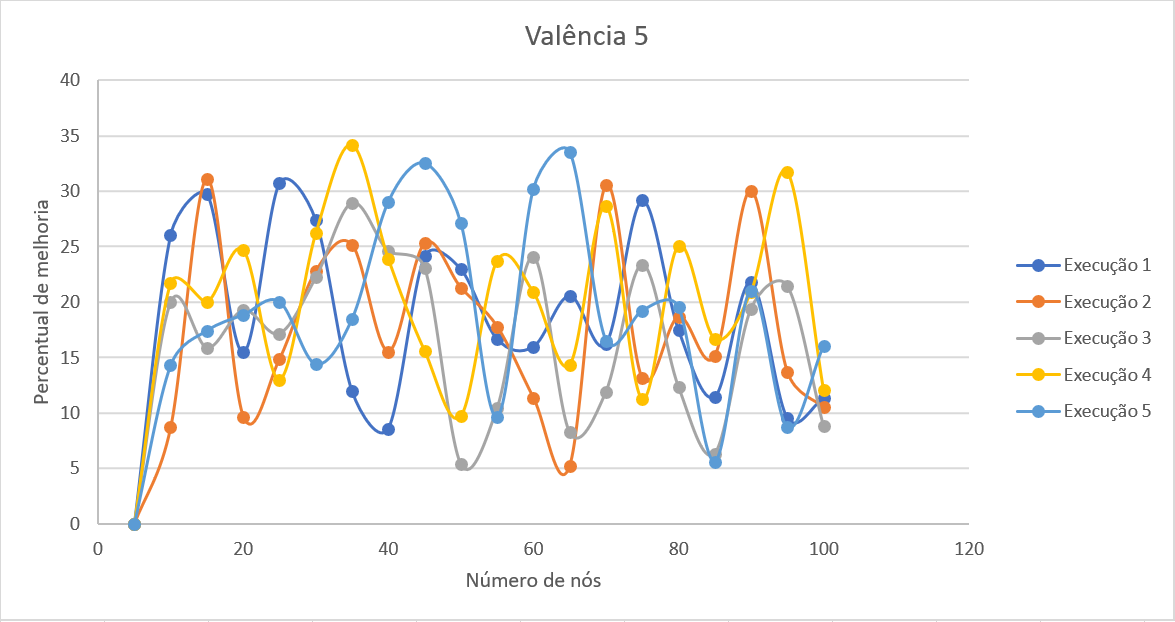
\includegraphics[width=8cm]{./figuras/BSN-valencia5-5exec-grafico.png} % <- formatos PNG, JPG e PDF
	%\caption{Valência máxima 5.}
	%\label{fig_graph_bsn_val5}
	%\end{subfigure}
	%\caption[Melhoria de custo máximo]{Percentual de melhoria no parâmetro de custo máximo da rede após aplicação do BSN variando a valência máxima do grafo}
	%\label{fig_graph_bsn_5exec_melhoria}
%\end{figure}

\begin{figure} [ht]% normalmente utilizar [!t]
	\centering
	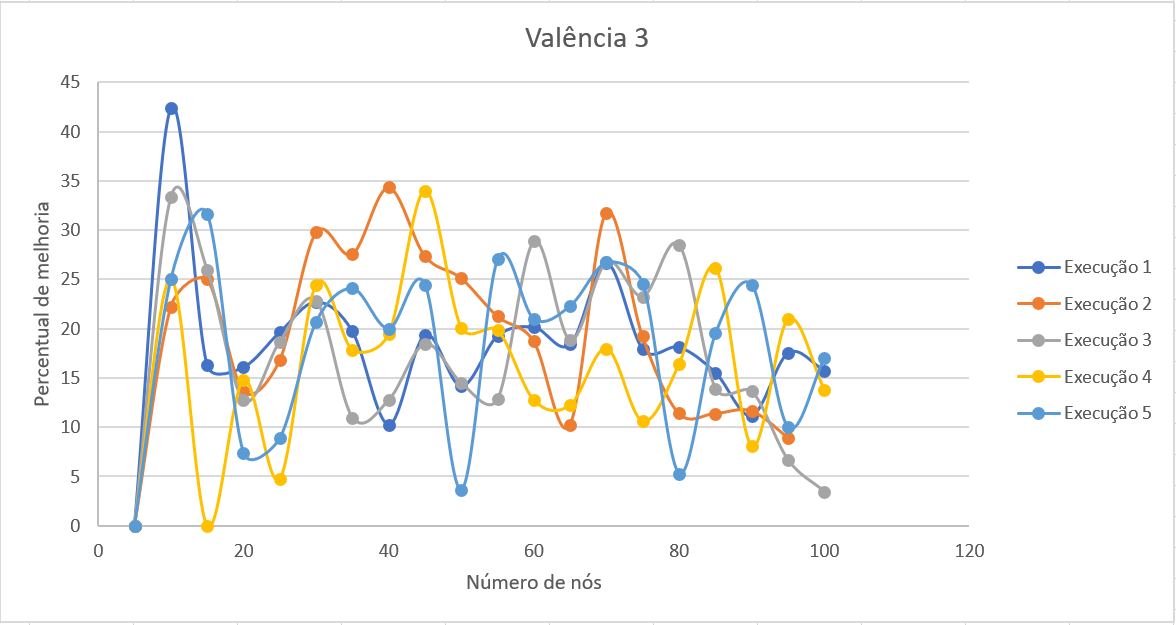
\includegraphics[width=0.8\textwidth]{./figuras/BSN-valencia3-5exec-grafico.png} % <- formatos PNG, JPG e PDF
		\caption[Melhoria de custo máximo com valência 3]{Percentual de melhoria no parâmetro de custo máximo da rede após aplicação do BSN considerando valência máxima 3.}
		\label{fig_graph_bsn_val3}
\end{figure}

\begin{figure} [ht]% normalmente utilizar [!t]
	\centering
	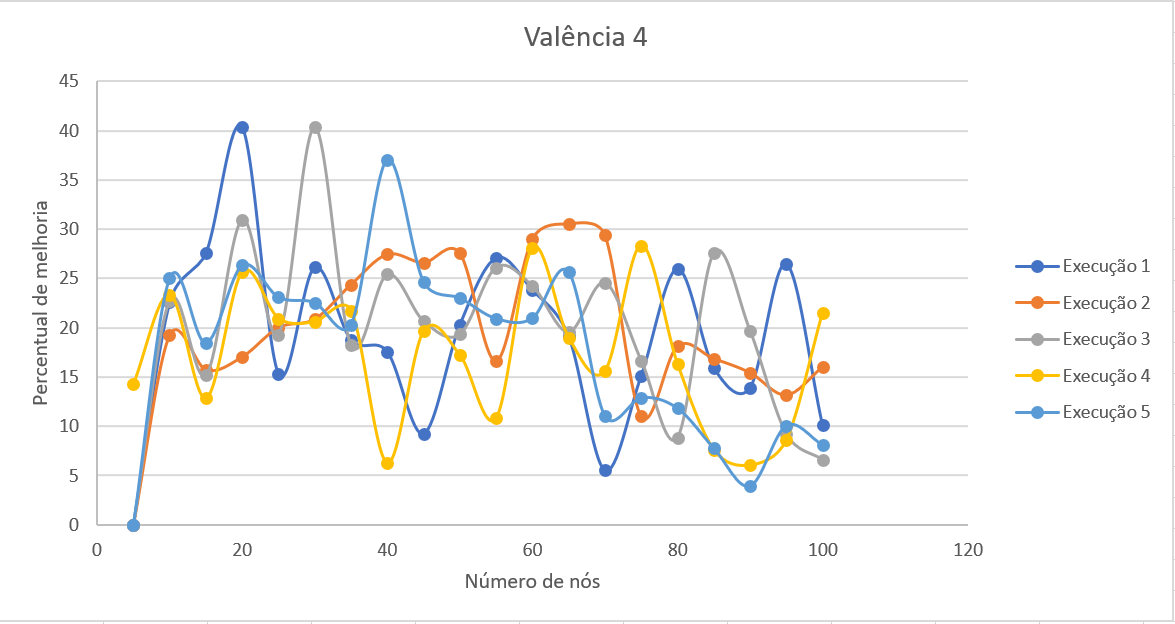
\includegraphics[width=0.8\textwidth]{./figuras/BSN-valencia4-5exec-grafico.png} % <- formatos PNG, JPG e PDF
		\caption[Melhoria de custo máximo com valência 4]{Percentual de melhoria no parâmetro de custo máximo da rede após aplicação do BSN considerando valência máxima 4.}
		\label{fig_graph_bsn_val4}
\end{figure}

\begin{figure} [ht]% normalmente utilizar [!t]
	\centering
	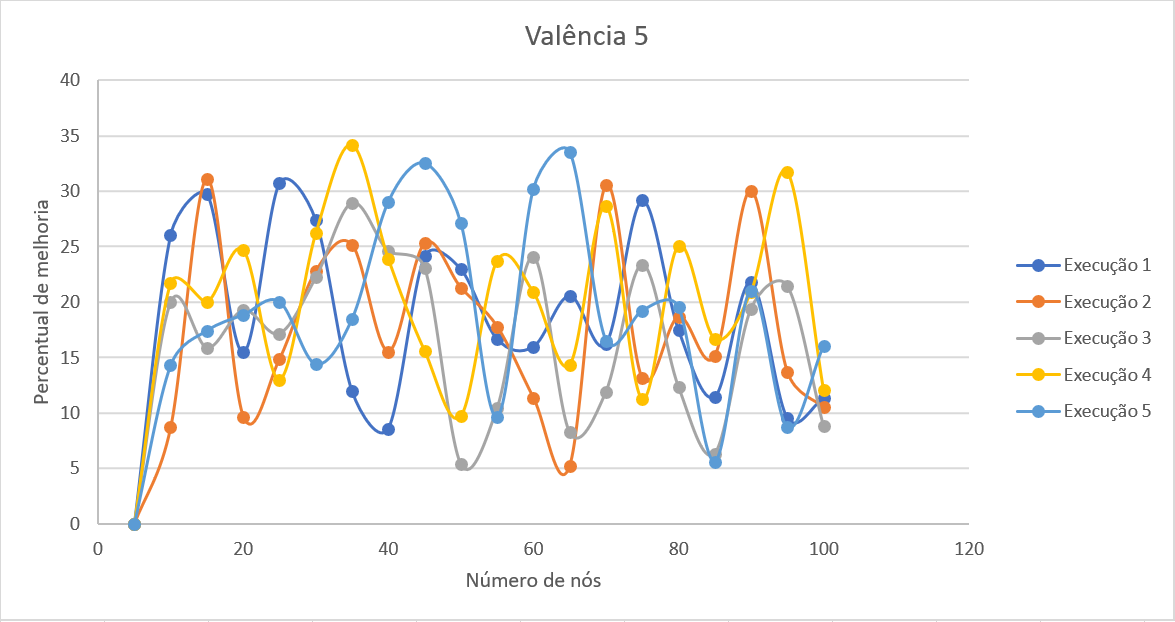
\includegraphics[width=0.8\textwidth]{./figuras/BSN-valencia5-5exec-grafico.png} % <- formatos PNG, JPG e PDF
	\caption[Melhoria de custo máximo com valência 5]{Percentual de melhoria no parâmetro de custo máximo da rede após aplicação do BSN considerando valência máxima 5.}
	\label{fig_graph_bsn_val5}
\end{figure}

Pode-se notar que para todos os casos os resultados de melhoria de percentual no custo total da rede tiveram grande variação, visto que as redes submetidas ao BSN foram completamente diferentes entre si. Desta forma pode-se afirmar que o comportamento do protocolo, como esperado, está intrinsecamente relacionado à topologia da rede original, visto que é esta topologia que irá gerar novos grafos quando do acionamento dos chaveadores ópticos. Sendo assim pode-se extrair, dentre todas as execuções, o pior e melhor caso de atuação do protocolo, representado na Figura \ref{fig_graph_bsn_pior_melhor}.

\begin{figure} [ht]% normalmente utilizar [!t]
	\centering
	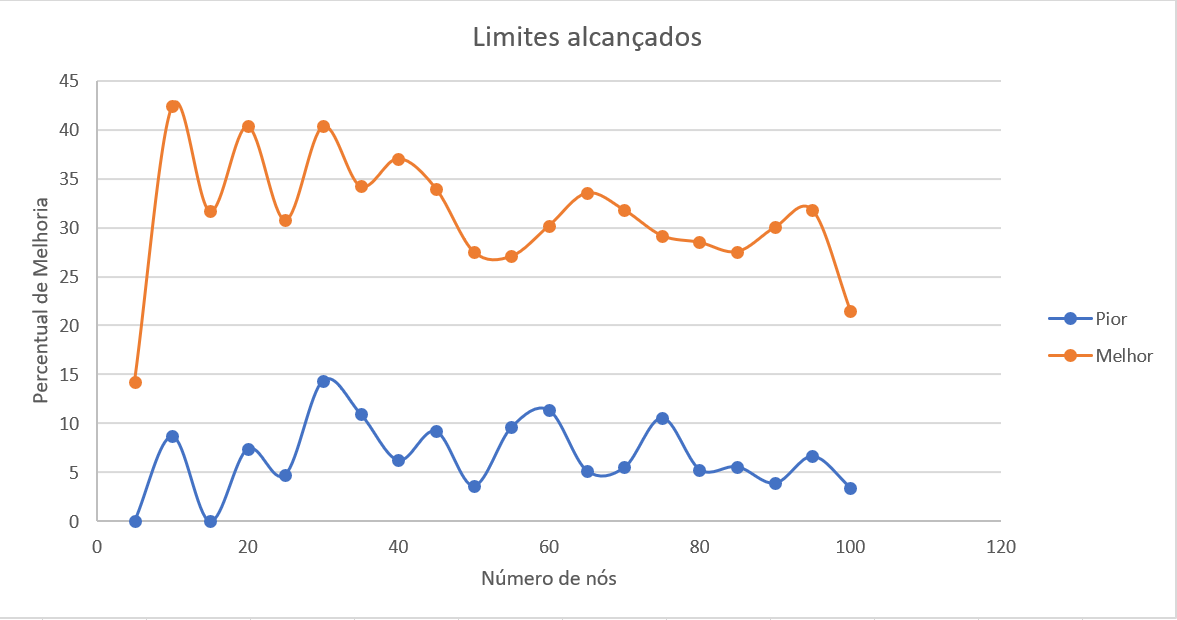
\includegraphics[width=0.8\textwidth]{./figuras/BSN-pior-melhor-exec.png} % <- formatos PNG, JPG e PDF
	\caption[Limites de melhoria alcançados]{Gráfico percentual comparativo entre os melhores e os piores resultados de melhoria alcançados utilizando o BSN.}
	\label{fig_graph_bsn_pior_melhor}
\end{figure}

Como pode-se perceber algumas redes avaliadas foram tão desfavoráveis à aplicação do BSN que não apresentaram nenhuma melhoria, este é o caso mostrado na curva da pior performance da Figura \ref{fig_graph_bsn_pior_melhor} para 5 e 15 nós. De maneira geral é fácil imaginar redes onde esse comportamento seja esperado, como aquelas em que não existam muitas redundâncias ou que eventualmente contenham grandes trechos em série (trechos com equipamentos que possam ser representados no grafo da rede por vértices de valência 2). Obviamente a probabilidade de se gerar uma rede como estas com um menor número de nós é muito maior do que considerando um grande número de nós, fato este que pode ser verificado no presente estudo visto que nenhuma rede maior apresentou o mesmo ``pior'' desempenho.

Em contrapartida, ainda analisando-se o gráfico da Figura \ref{fig_graph_bsn_pior_melhor}, pode-se notar um percentual de melhoria extremamente alto para redes propícias a multipercursos, podendo chegar em alguns a casos a níveis ao redor de 45\% de melhoria considerando-se o custo total da rede antes e depois da utilização do BSN. %falar sobre res medios e tamanho da rede

A Figura \ref{fig_graph_bsn_medio} mostra os resultados médios obtidos com os resultados das mesmas 5 execuções software de simulação que geraram as Figuras \ref{fig_graph_bsn_val3} a \ref{fig_graph_bsn_val5}. Como pode-se observar o desempenho do BSN é muito mais afetado pelo número de nós do que pela valência máxima do grafo utilizado.

\begin{figure} [ht]% normalmente utilizar [!t]
	\centering
	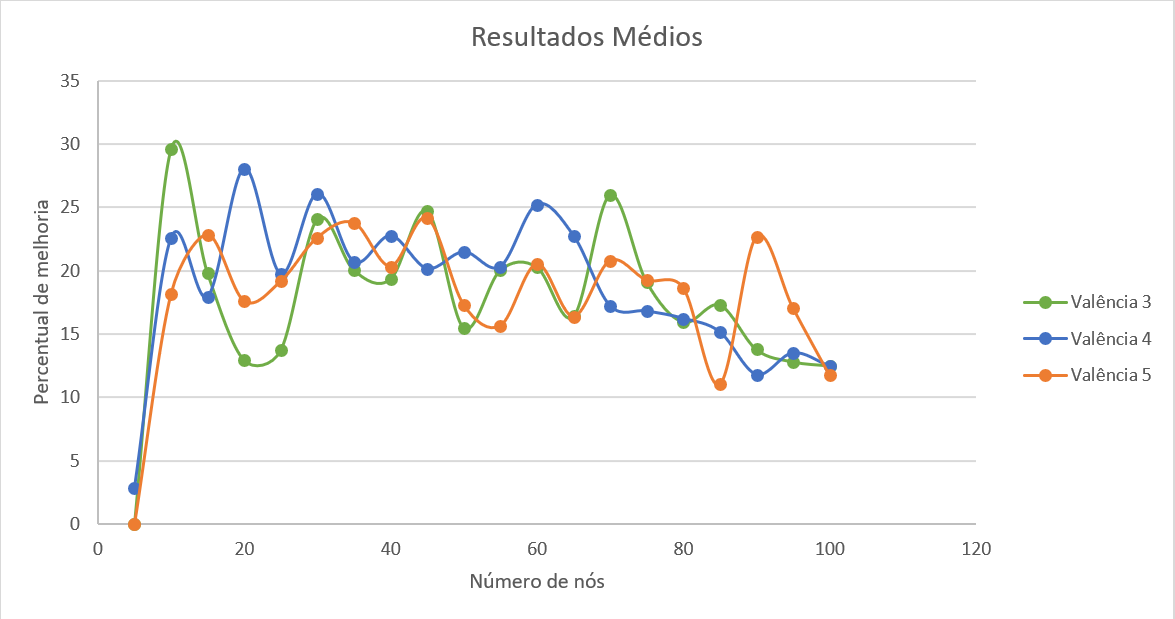
\includegraphics[width=0.8\textwidth]{./figuras/BSN-resultados-medios.png} % <- formatos PNG, JPG e PDF
	\caption[Melhoria de custo x valência]{Gráfico percentual comparativo de resultados médios de melhoria de custo total entre redes de diferentes valências.}
	\label{fig_graph_bsn_medio}
\end{figure}

Baseando-se na conclusão de que a influência da valência no desempenho do BSN não é relevante pode-se gerar um gráfico que mostre o percentual de melhoria de custo total considerando apenas o número de nós das redes avaliadas. Para isso foram utilizadas 300 redes diferentes resultando no representado na Figura \ref{fig_graph_bsn_medio_all}. Aqui fica claro uma diminuição no percentual de melhoria com o aumento do número de nós da rede utilizada. 

\begin{figure} [ht]% normalmente utilizar [!t]
	\centering
	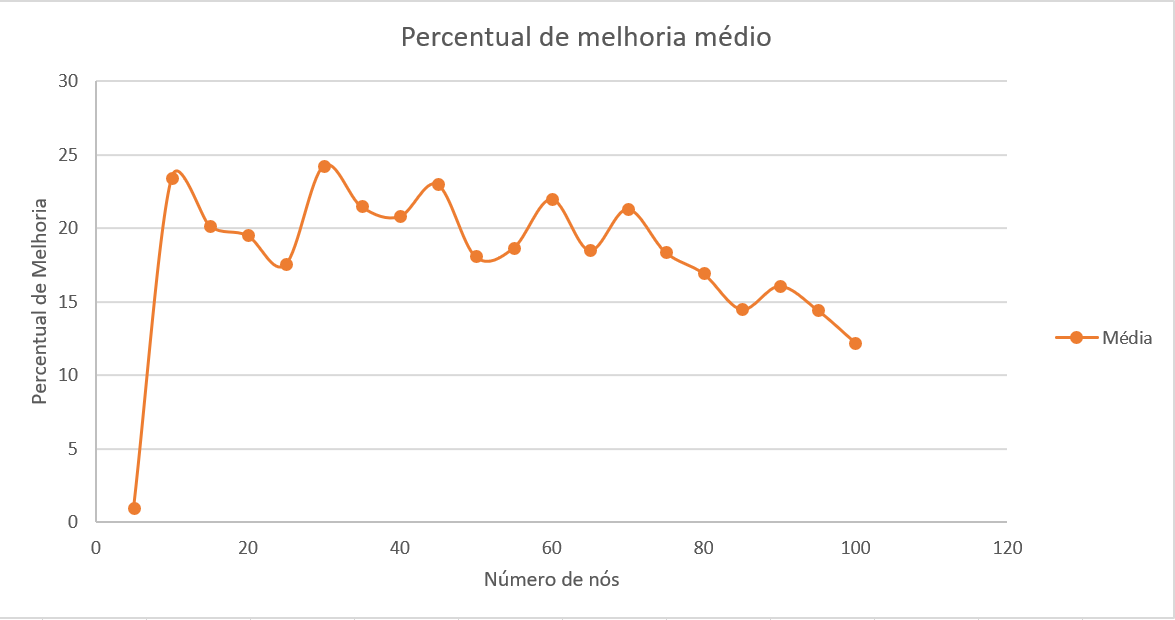
\includegraphics[width=0.8\textwidth]{./figuras/BSN-resultados-medios-all.png} % <- formatos PNG, JPG e PDF
	\caption[Melhoria de custo x tamanho de rede]{Gráfico percentual comparativo de resultados médios de melhoria de custo total entre redes de diferentes tamanhos.}
	\label{fig_graph_bsn_medio_all}
\end{figure}

\subsection{Melhoria de custo Individual}
Conforme explicitado em \ref{subsection-custo-da-rede}, além de significativa melhora no custo total da rede, o BSN apresenta um ótimo resultado ao avaliar-se o custo individual para comunicação entre o nó central e cada um dos demais.

\subsection{Limitações}
Comentar sobre estar usando apenas um optsw e sobre a opcao única de ligar a primeira fibra na ultima


%\chapter{Desenvolvimento}
%\label{chap:desenv}
%
%A seguir ilustra-se a forma de incluir figuras, tabelas, equa\c{c}\~oes, siglas e s\'imbolos no documento, obtendo indexa\c{c}\~ao autom\'atica em suas respectivas listas. A numera\c{c}\~ao sequencial de figuras, tabelas e equa\c{c}\~oes ocorre de modo autom\'atico. Refer\^encias cruzadas s\~ao obtidas atrav\'es dos comandos {\ttfamily \textbackslash label\{\}} e {\ttfamily \textbackslash ref\{\}}. Por exemplo, n\~ao \'e necess\'ario saber que o n\'umero deste cap\'itulo \'e~\ref{chap:desenv} para colocar o seu n\'umero no texto. Isto facilita muito a inser\c{c}\~ao, remo\c{c}\~ao ou reloca\c{c}\~ao de elementos numerados no texto (fato corriqueiro na escrita e corre\c{c}\~ao de um documento acad\^emico) sem a necessidade de renumer\'a-los todos.
%
%\section{Figuras}
%
%Na figura~\ref{fig:dummy} \'e apresentado um exemplo de gr\'afico flutuante. Esta figura aparece automaticamente na lista de figuras. Para uso avan\c{c}ado de gr\'aficos no \LaTeX, recomenda-se a consulta de literatura especializada~\cite{Goossens2007}.
%
%
%\begin{figure}[!htb]
	%\centering
	%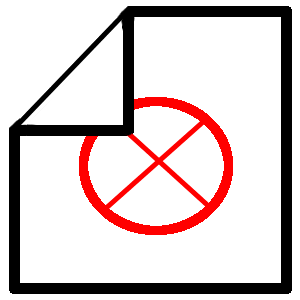
\includegraphics[width=0.2\textwidth]{./figuras/dummy.png} % <- formatos PNG, JPG e PDF
	%\caption[Exemplo de uma figura]{Exemplo de uma figura onde aparece uma imagem sem nenhum significado especial.}
	%\fonte{\cite{abnTeX2009}}
	%\label{fig:dummy}
%\end{figure}
%
%
%\section{Tabelas}
%
%Tamb\'em \'e apresentado o exemplo da tabela~\ref{tab:correlacao}, que aparece automaticamente na lista de tabelas. Informa\c{c}\~oes sobre a constru\c{c}\~ao de tabelas no \LaTeX\ podem ser encontradas na literatura especializada~\cite{Lamport1986,Buerger1989,Kopka2003,Mittelbach2004}.
%
%\begin{table}[!htb]
	%\centering
	%\caption[Exemplo de uma tabela]{Exemplo de uma tabela mostrando a correla\c{c}\~ao entre x e y.}
	%\label{tab:correlacao}
	%\begin{tabular}{cc}
		%\hline 
		%x & y \\
		%\hline
		%1 & 2 \\
		%3 & 4 \\
		%5 & 6 \\
		%7 & 8 \\
		%\hline 
	%\end{tabular}
	%\fonte{Autoria pr\'opria.}
%\end{table}
%
%\section{Equa\c{c}\~oes}
%
%A transformada de Laplace \'e dada na equa\c{c}\~ao~(\ref{eq:laplace}), enquanto a equa\c{c}\~ao~(\ref{eq:dft}) apresenta a formula\c{c}\~ao da transformada discreta de Fourier bidimensional\footnote{Deve-se reparar na formata\c{c}\~ao esteticamente perfeita destas equa\c{c}\~oes!}.
%
%\begin{equation}
%X(s) = \int\limits_{t = -\infty}^{\infty} x(t) \, \text{e}^{-st} \, dt
%\label{eq:laplace}
%\end{equation}
%
%\begin{equation}
%F(u, v) = \sum_{m = 0}^{M - 1} \sum_{n = 0}^{N - 1} f(m, n) \exp \left[ -j 2 \pi \left( \frac{u m}{M} + \frac{v n}{N} \right) \right]
%\label{eq:dft}
%\end{equation}
%
%\section{Siglas e s\'imbolos}
%
%O pacote \textsc{abn}\TeX\ permite ainda a defini\c{c}\~ao de siglas e s\'imbolos com indexa\c{c}\~ao autom\'atica atrav\'es dos comandos {\ttfamily \textbackslash sigla\{\}\{\}} e {\ttfamily \textbackslash simbolo\{\}\{\}}. Por exemplo, o significado das siglas\sigla{CPGEI}{Programa de P\'os-gradua\c{c}\~ao em Engenharia El\'etrica e Inform\'atica Industrial},\sigla{DAELN}{Departamento Acad\^emico de Eletr\^onica} e\sigla{UTFPR}{Universidade Tecnol\'ogica Federal do Paran\'a} aparecem automaticamente na lista de siglas, bem como o significado dos s\'imbolos\simbolo{$\lambda$}{comprimento de onda},\simbolo{$v$}{velocidade} e\simbolo{$f$}{frequ\^encia} aparecem automaticamente na lista de s\'imbolos. Mais detalhes sobre o uso destes e outros comandos do \textsc{abn}\TeX\ s\~ao encontrados na sua documenta\c{c}\~ao espec\'ifica~\cite{abnTeX2009}.


%---------- Terceiro Capitulo ----------
\chapter{Conclus\~ao}

%Espera-se que o uso do estilo de formata\c{c}\~ao \LaTeX\ adequado \`as Normas para Elabora\c{c}\~ao de Trabalhos Acad\^emicos da UTFPR ({\ttfamily normas-utf-tex.cls}) facilite a escrita de documentos no \^ambito desta institui\c{c}\~ao e aumente a produtividade de seus autores. Para usu\'arios iniciantes em \LaTeX, al\'em da bibliografia especializada j\'a citada, existe ainda uma s\'erie de recursos~\cite{CTAN2009} e fontes de informa\c{c}\~ao~\cite{TeX-Br2009,Wikibooks2009} dispon\'iveis na Internet.
%
%Recomenda-se o editor de textos Kile como ferramenta de composi\c{c}\~ao de documentos em \LaTeX\ para usu\'arios Linux. Para usu\'arios Windows recomenda-se o editor \TeX nicCenter~\cite{TeXnicCenter2009}. O \LaTeX\ normalmente j\'a faz parte da maioria das distribui\c{c}\~oes Linux, mas no sistema operacional Windows \'e necess\'ario instalar o software \textsc{MiK}\TeX~\cite{MiKTeX2009}.
%
%Al\'em disso, recomenda-se o uso de um gerenciador de refer\^encias como o JabRef~\cite{JabRef2009} ou Mendeley~\cite{Mendeley2009} para a cataloga\c{c}\~ao bibliogr\'afica em um arquivo \textsc{Bib}\TeX, de forma a facilitar cita\c{c}\~oes atrav\'es do comando {\ttfamily \textbackslash cite\{\}} e outros comandos correlatos do pacote \textsc{abn}\TeX. A lista de refer\^encias deste documento foi gerada automaticamente pelo software \LaTeX\ + \textsc{Bib}\TeX\ a partir do arquivo {\ttfamily reflatex.bib}, que por sua vez foi composto com o gerenciador de refer\^encias JabRef.
%
%O estilo de formata\c{c}\~ao \LaTeX\ da UTFPR e este exemplo de utiliza\c{c}\~ao foram elaborados por Diogo Rosa Kuiaski (diogo.kuiaski@gmail.com) e Hugo Vieira Neto (hvieir@utfpr.edu.br), com contribui\c{c}\~oes de C\'esar Vargas Benitez. Sugest\~oes de melhorias s\~ao bem-vindas.


%---------- Referencias ----------
\clearpage % this is need for add +1 to pageref of bibstart used in 'ficha catalografica'.
\label{bibstart}
\bibliography{referencias,SMMC2018} % geracao automatica das referencias a partir do arquivo reflatex.bib
\label{bibend}

%---------- Apendices (opcionais) ----------
%\apendice
%\chapter{Nome do Ap\^endice}
%
%Use o comando {\ttfamily \textbackslash apendice} e depois comandos {\ttfamily \textbackslash chapter\{\}}
%para gerar t\'itulos de ap\^en-dices.
%
%
%% ---------- Anexos (opcionais) ----------
%\anexo
%\chapter{Nome do Anexo}
%
%Use o comando {\ttfamily \textbackslash anexo} e depois comandos {\ttfamily \textbackslash chapter\{\}}
%para gerar t\'itulos de anexos.


% --------- Ordenacao Afabetica da Lista de siglas --------
%\textbf{* Observa\c{c}\~oes:} a ordenacao alfabetica da lista de siglas ainda nao eh realizada de forma automatica, porem
% eh possivel se de realizar isto manualmente. Duas formas:
%
% ** Primeira forma)
%    A ordenacao eh feita com o auxilio do comando 'sort', disponivel em qualquer
% sistema Linux e UNIX, e tambem em sistemas Windows se instalado o coreutils (http://gnuwin32.sourceforge.net/packages/coreutils.htm)
% comandos para compilar e ordenar, supondo que seu arquivo se chame 'dissertacao.tex':
%
%      $ latex dissertacao
%      $ bibtex dissertacao && latex dissertacao
%      $ latex dissertacao
%      $ sort dissertacao.lsg > dissertacao.lsg.tmp
%      $ mv dissertacao.lsg.tmp dissertacao.lsg
%      $ latex dissertacao
%      $ dvipdf dissertacao.dvi
%
%
% ** Segunda forma)
%\textbf{Sugest\~ao:} crie outro arquivo .tex para siglas e utilize o comando \sigla{sigla}{descri\c{c}\~ao}.
%Para incluir este arquivo no final do arquivo, utilize o comando \input{arquivo.tex}.
%Assim, Todas as siglas serao geradas na ultima pagina. Entao, devera excluir a ultima pagina da versao final do arquivo
% PDF do seu documento.


%-------- Citacoes ---------
% - Utilize o comando \citeonline{...} para citacoes com o seguinte formato: Autor et al. (2011).
% Este tipo de formato eh utilizado no comeco do paragrafo. P.ex.: \citeonline{autor2011}

% - Utilize o comando \cite{...} para citacoeses no meio ou final do paragrafo. P.ex.: \cite{autor2011}



%-------- Titulos com nomes cientificos (titulo, capitulos e secoes) ----------
% Regra para escrita de nomes cientificos:
% Os nomes devem ser escritos em italico, 
%a primeira letra do primeiro nome deve ser em maiusculo e o restante em minusculo (inclusive a primeira letra do segundo nome).
% VEJA os exemplos abaixo.
% 
% 1) voce nao quer que a secao fique com uppercase (caixa alta) automaticamente:
%\section[nouppercase]{\MakeUppercase{Estudo dos efeitos da radiacao ultravioleta C e TFD em celulas de} {\textit{Saccharomyces boulardii}}
%
% 2) por padrao os cases (maiusculas/minuscula) sao ajustados automaticamente, voce nao precisa usar makeuppercase e afins.
% \section{Introducao} % a introducao sera posta no texto como INTRODUCAO, automaticamente, como a norma indica.


\end{document}
